\documentclass[11pt]{article}

%%%%%%%%%%%%      PACKAGES        %%%%%%%%%%%%
\usepackage[colorlinks=true,linkcolor=blue,urlcolor=blue,citecolor=blue]{hyperref}
\usepackage{setspace}
\onehalfspacing
%\doublespacing
\usepackage{fancyhdr,afterpage}
\usepackage{lscape}
\usepackage{multirow}
\usepackage{longtable}
\usepackage{textcomp,latexsym}
\usepackage{parskip}
\usepackage[round]{natbib}
\usepackage{adjustbox,lipsum}
\usepackage[titletoc]{appendix}
    
\usepackage[round]{natbib}
\usepackage{amsmath}
\usepackage{graphicx}
\usepackage{gensymb}
\usepackage{tikz}
\usepackage{float}
%\usepackage{slashbox}
\usepackage{caption}
\usepackage{subcaption}
\usepackage{amsfonts}
\usepackage{enumerate}
\usepackage{amssymb}
\usepackage{multirow}
\usepackage{bm}
\setcounter{tocdepth}{3}
\setcounter{secnumdepth}{3}

\DeclareMathOperator*{\argmax}{arg\,max}
\DeclareMathOperator*{\argmin}{arg\,min}

\usepackage[a4paper,inner=4.2cm,outer=2.3cm,top=2.5cm,bottom=2.5cm,pdftex]{geometry} % MARGINS


\begin{document}
\tableofcontents

\newpage
\section{Abstract}

\section{Introduction}

\begin{Large}
	
\end{Large}

Most experiments are conducted in order to gain understanding of the impact that different parameters of interest make on the outcome; the quantitative measure of this impact allows comparisons as well as making interpretable conclusions regarding the scale and the pattern of the relationships between process parameters and measured output. 
%% Polynomial models
While the exact true nature of that relationship remains unknown, we need to have some form of approximation. Polynomial functions are well known to be able to provide an approximation of any required precision for functions from a certain class of differentiability \citep{Rudin1987real}: obviously, higher desirable precision would require a polynomial of a higher order and, therefore, more experimental effort. Response Surface Methodology (RSM) that was first introduced by \cite{Box1951Roy} is aimed at optimising the response by fitting a second order polynomial to the data obtained after an experiment on the points within the experimental region of interest has been performed. The response measured at each of $n$ experimental runs would then be presented as a linear combination of experimental factors' values, their interactions and corresponding quadratic terms; of course, some of the terms might be excluded, but, unless stated otherwise, we will consider a full second-order polynomial model with $1+2k+\frac{k(k-1)}{2}$ parameters (including the intercept), where $k$ is the number of factors. Together with the fixed polynomial part, the error term here would stand for all the variation in data that has not been captured by the model. 
%% Experimental design
At the stage of experimental planning, when there is little, if any, prior knowledge and no data available, there is still a lot that can and should be done to make sure the results of the experimentation and the following analysis are credible.

The design construction usually depends on the model in several ways. Firstly, the interest in the properties of the model parameters' estimation leads to the development of various optimality criteria (e.g.~so-called `alphabetic criteria'). Secondly, the fact of the model-dependence of the majority of the criteria implies the necessity of taking into account the possible lack-of-fit as well as the desirability of obtaining error variance estimates from replicated observations (model-independent, `pure' error). The latter two are also in the list of the properties of what would be considered as a `good design' (summarised by \cite{Box1987empirical}, Chapter $14$): it should ``make it possible to detect lack of fit'' and ``provide an internal estimate of error from replication''.

It is obvious that all the individual criteria are not interchangeable and can possibly be contradictory, however, they all are desired to be accounted for. There are a few ways of combining them, and here we will be working with the notion of a compound optimality criterion which is basically a weighted combination of the elementary criteria, where weights are generally arbitrary, and are expected to be chosen in accordance with the experimenter's beliefs and intentions. 

We will focus in this work on factorial experiments with a relatively small number of runs and the fitted model being a polynomial regression. We work here with exact designs: for each run we are to provide a point as a combination of the treatment factors' levels; therefore, finding the corresponding optimal design is essentially a matrix optimisation problem, i.e. searching for a design maximising (minimising) the criterion function. When considering examples of different compound criteria with various weight allocations, we will examine the resulting optimal designs in terms of their performances with respect to individual components. This would allow evaluating how much is ``lost'' when achieving a compromise, what component criteria contradict each others' performances, and how they are affected by changes of weight allocations.

The first and main objective of the research presented is to develop a methodology for combining several desirable data inference properties in compound optimality criteria for factorial experiments. The properties are to correspond to the precision of inference based on the primary model and to the possibility of the specified model contamination presence; the components are aimed to comply with the `pure error' strategy, where it is feasible.

The obvious following objective is to investigate the relationships between the individual components of the introduced criteria and, by considering some examples, provide some empirical recommendations for complex experimentation research that would benefit from applying these methods.

The criteria will also be adapted to be applied within experimental frameworks with restricted randomisation: blocked and multistratum experiments.

\section{Background}

Recall the polynomial regression model (\ref{eq::back_model}) for the unblocked experiment, containing initial factors, their powers and interactions is used as a good approximation to the relation between the variables:  

\begin{equation}
\label{eq::back_model}
\bm{Y}=\bm{X\beta}+\bm{\varepsilon}.
\end{equation} 

Here $\bm{X}$ is the $n\times p$ model matrix, $\bm{Y}$ is the $n\times 1$ vector of responses; $\bm{\beta}$ is the $p\times 1$ vector of parameters corresponding to the model terms and $\bm{\varepsilon}$ are independent normally distributed random error terms with constant variance, i.e. $\bm{\varepsilon}\sim \mathcal{N}(\bm{0},\sigma^{2}\bm{I}_{n})$.

\subsection{Error estimation}
The error variance estimation can be obtained in two ways. The first one is the mean square error: $\hat{\sigma}^2_{mse}=\mbox{Residual SS}/(n-p)$, i.e. the residual sum of squares divided by the corresponding number of degrees of freedom (obtained from the ANOVA decomposition, the details can be found in \cite{Draper1998}). This estimator obviously depends on the model and on the number of its parameters. The other one is model-independent `pure' error, derived from the further decomposition of the residual sum of squares into the `pure' error and `lack-of-fit' components: $\hat{\sigma}^2_{PE}=\mbox{Pure error SS}/(n-t)$, where $t$ is the number of unique treatments applied and $d=n-t$ is the pure error degrees of freedom, i.e. the number of replicated points. In other words, the error is estimated by fitting the full treatment model:

\begin{equation}
\label{eq::back_trnt}
\bm{Y}=\bm{X_{t}\mu_{t}}+\bm{\varepsilon},
\end{equation} 

where $\bm{X_{t}}$ is the $n\times t$ full treatment model matrix, in which the $(i,j)^{th}$ element is equal to $1$ if treatment $j$ is applied to the $i^{th}$ unit, otherwise it is set to $0$. Then the elements of the $t$-dimensional vector $\bm{\mu_{t}}$ are the mean effects of each treatment. The vector of errors $\bm{\varepsilon}$ comprises the between-unit variation, such that $\mbox{E}(\bm{\varepsilon})=\bm{0}$, $\mbox{Var}(\bm{\varepsilon})=\sigma^2\bm{I}_{n}$.

Many authors advocate the use of the `pure' error estimate of $\sigma^2$ instead of the one pooled with the lack-of-fit part from the model (\ref{eq::back_model}): \cite{Cox1958planning} recommends using it for the estimation unless there are no replicate treatments, while \cite{Draper1998} argue for the reliability of `pure' error and recommend aiming for the presence of replicates at the stage of planning. \cite{Atkinson2007} also state that ``If lack-of-fit of the model is of potential interest, $\sigma^{2}$ is better estimated from replicate observations'' (page 22). For response surface experiments in blocks \cite{Gilmour2000PErsm} explicated the definition of pure error and its estimate which are compatible with the unblocked case: from replicates but also taking into account  block effects additive to treatment effects. Finally, the work by \cite{GilmourTrinca2012} that inspired this research, comprises a thorough analysis in favour of estimating the error from the full treatment model which is true regardless of what function is used to approximate the relationship of interest.

?? Adding background on MS experiments: briefly about the structure, pure-error reml, note on degresof freedom. 

\subsection{Combining criteria}

The concept of the compound criteria is based on the notion of design efficiency, which can be defined for any design matrix and any criterion. For example, the $D$-efficiency of design $\bm{X}$ is
\begin{equation}
\label{eq::D_eff}
\mbox{Eff}_{D}(X)=\left[\frac{\vert \bm{X}'\bm{X}\vert}{\vert \bm{X}'_{*}\bm{X}_{*}\vert}\right]^{1/p},
\end{equation}   
where $\bm{X}_{*}$ is the $D$-optimum design. In this definition the power $1/p$ brings the efficiency to the scale of variances of model coefficients $\bm{\beta}_{i}, i=1\ldots p.$ It is obvious that the efficiency value may vary from $0$ to $1$ and is equal to $1$ if and only if the design is optimal according to the criterion of interest.

The final criterion function to be maximised among all the possible designs is obtained by combining the efficiencies for the component criteria $\mbox{Eff}_{1},\ldots, \mbox{Eff}_{m}$ with the corresponding weights $\kappa_{1},\ldots ,\kappa_{m}$ such that each $\kappa_{k}>0$ and $\sum_{k=1}^{m}\kappa_{k}=1:$

\begin{equation}
\label{eq::compound}
\mbox{Eff}^{\kappa_{1}}_{1}(\bm{X})\times\mbox{Eff}^{\kappa_{2}}_{2}(\bm{X})\times\ldots\times\mbox{Eff}^{\kappa_{m}}_{m}(\bm{X})\rightarrow \underset{\bm{X}}\max.
\end{equation}

The choice of weights is an arbitrary decision, made relying on both prior knowledge of the experimenter, the objectives of a specific experiment and the interpretation of the criterion components. The most general and intuitively sensible recommendation would be to obtain optimal designs with respect to several weight allocations, and then, after examining them, choose the one to be applied. Throughout the course of this research, when considering the examples of experiments layouts, we chose a set of weight allocations. Most of these sets were essentially classical design schemes for experiments with mixtures \citep{Cornell2011Mixtures}. For example, if the criterion consists of three elements, we would first obtain designs with all the weight on each component, then all combinations of distributing it equally between two components, and finally put equal weights on all of the components. Some additional schemes are included when examining particular cases.  

Some of the alternative approaches of considering several objectives would include the Pareto frontier approach, thoroughly described, for example, by \cite{Lu2011optimization}. When there are $l$ individual criterion functions $\phi_1(\bm{X}),\ldots\phi_{l}(\bm{X})$ to be maximised, the Pareto optimal set is generated so that for each of the designs from this set there is no other possible design that provides better criterion values for all the criteria (or, as it was defined, the Pareto optimal set is formed of designs that are not ``dominated'' by any other design).

Another approach was presented by \cite{Stallings2015general}: the authors developed methodology for generalising eigenvalue-based criteria (e.g. $A$- and $E$-optimality) in a way that allows differing interest (expressed through the weights) among any set of estimable functions of the fitted model parameters. The introduced strategy reflects the aims of experimentation that are not traditionally accounted for but definitely are of interest.

\section{Individual criteria construction}
\label{ch::compound_criteria}
Standard design optimality theory is developed under the assumption that the fitted model represents the true relationship of interest and that there is no misspecification. However, it is obviously quite a strong belief and in reality we need to take into account at least the possibility that the model might not provide a good fit to the data. In Section \ref{sec::back_misspecification} a brief overview of various types of model misspecification is presented. 

In this chapter we consider the case when the fitted polynomial model is nested within a larger model that is assumed to provide a better fit for the data:
\begin{equation}
\label{eq::full_model}
\bm{Y}=\bm{X}_1\bm{\beta}_1+\bm{X}_2\bm{\beta}_2+\bm{\varepsilon},
\end{equation}
where $\bm{X}_2$ is an $n\times q$ is an extension of the initial model matrix representing those extra $q$ potential terms that might represent the fitted model disturbance. The vector $\bm{\beta}_2$ denotes the corresponding parameters. This larger model has $p+q$ parameters in total and not all of them are estimable when the experiment is relatively small: $n<p+q$; this is the case we consider here.
\subsection{Lack-of-fit criterion}
We consider the Generalised criterion presented by Goos et al.: [more details?]
\begin{equation*}
\mbox{minimise }|\bm{X}'_{1}\bm{X}_1|^{-\frac{\kappa_{D}}{p}}\times \left|\bm{L}+\frac{\bm{I}_{q}}{\tau^{2}}\right|^{-\frac{\kappa_{LoF}}{q}} \times |\bm{A}'\bm{A}+\bm{I}_{q}|.^{\frac{\kappa_{bias}}{q}},
\end{equation*}
where $\bm{L}$ is known in literature as dispersion matrix, and the matrix $\bm{L}+\bm{I}_{q}/\tau^{2}$ in the second component is essentially the inverse posterior variance-covariance matrix of the vector of potential terms (up to a factor of $\sigma^2$).

 ** Derivation first or the Generalised criterion

A diffuse prior shall be put on primary terms (as was done by \cite{DuMouchel1994}) -- an arbitrary mean and a variance going to infinity, and the prior on potential terms is the one specified before: $\bm{\beta}_2\sim\mathcal{N}(0,\bm{\Sigma}_{0})$,
$\bm{\Sigma}_{0}=\sigma^{2}\tau^{2}\bm{I}_{q}$, then the posterior
distribution of the coefficients is (as in \cite{Koch2007introduction} and \cite{DuMouchel1994}):
$$\bm{\beta}|\bm{Y}\sim \mathcal{N}(\bm{b},\bm{\Sigma}),\mbox{ where }\bm{b}=\bm{\Sigma X}'\bm{Y}, \bm{X}=[\bm{X}_1, \bm{X}_2],$$
$$\bm{\Sigma}=\left[\frac{\bm{K}}{\sigma^{2}\tau^{2}}+\sigma^{-2}(\bm{X'X})\right]^{-1}=\sigma^{2}[\bm{K}/\tau^{2}+\bm{X'}\bm{X}],^{-1}$$
and 
\begin{equation*}
\bm{K}=\begin{pmatrix}
\bm{0}_{p\times p} & \bm{0}_{p\times q}\\
\bm{0}_{q\times p} & \bm{I}_{q\times q}
\end{pmatrix}.
\end{equation*}
The marginal posterior of $\bm{\beta}_2$ is $\mathcal{N}(\bm{b}_{2},\bm{\Sigma}_{22})$, so using the general formula for the inverse of a block matrix
$$\begin{bmatrix}
 \bm{A}& \bm{B}\\
 \bm{C}& \bm{D}
\end{bmatrix}^{-1}=\begin{bmatrix}
\ldots & \ldots\\
\ldots & (\bm{D}-\bm{CA}^{-1}\bm{B})^{-1}
\end{bmatrix},$$
we can obtain the expression for $\bm{\Sigma}_{22}$:
\begin{align*}
[\bm{K}/\tau^{2}+\bm{X}'\bm{X}]^{-1}&=\begin{bmatrix}
 \bm{X}'_1\bm{X}_1& \bm{X}'_1\bm{X}_2 \\
 \bm{X}'_2\bm{X}_1& \bm{X}'_2\bm{X}_2+\bm{I}_{q}/\tau^{2}
\end{bmatrix}^{-1}\\&=\begin{bmatrix}
\ldots & \ldots\\
\ldots &
(\bm{X}'_2\bm{X}_2+\bm{I}_{q}/\tau^{2}-\bm{X}'_2\bm{X}_1(\bm{X}'_1\bm{X}_1)^{-1}\bm{X}'_1\bm{X}_2)^{-1}
\end{bmatrix},\\
\bm{\Sigma}_{22}&=\sigma^{2}[(\bm{K}/\tau^{2}+\bm{X}^{'}\bm{X})^{-1}]_{22}=\sigma^{2}\left(\bm{L}+\frac{\bm{I}_{q}}{\tau^{2}}\right)^{-1},
\end{align*} 
and $$(\bm{\Sigma}_{22})^{-1}=\frac{1}{\sigma^{2}}\left(\bm{L}+\frac{\bm{I}_{q}}{\tau^{2}}\right).$$

Therefore, the $(1-\alpha)\times100\%$ confidence region for the potential terms over the posterior distribution, when $\sigma^2$ is estimated by $s^2$ on $\nu$ degrees of freedom, is given by \citep{Draper1998}:

$$(\bm{\beta}_{2}-\bm{b}_{2})^{'}(\bm{L}+\bm{I}_{q}/\tau^{2})(\bm{\beta}_{2}-\bm{b}_{2})\leq qs^{2}F_{q,\nu;1-\alpha},$$
where $\mathrm{F}(q,\nu,\alpha)$ is the $\alpha$-quantile of F-distribution with $q$ and $\nu$ degrees of freedom.\\ 

\subsection{MSE-based bias criterion}
From the inference point of view, in the case of potential model contamination the bias in the parameters' estimates would be of substantial interest. A natural way of evaluating the quality of $\bm{\hat{\beta}}_{1}$, as noted by \citet{FedorovMontepiedra1997} is the matrix of  mean square error, which is the $\bm{L}_2$-distance between the true and estimated values with respect to the probability distribution measure of $\bm{Y}$ under the assumption of model (\ref{eq::full_m}):
\begin{align}
\label{eq::MSE}
\mbox{MSE}(\bm{\hat{\beta}}_1|\bm{\beta})=&\mathtt{E}_{\bm{Y}|\bm{\beta}}[(\bm{\hat{\beta}}_1-\bm{\beta}_1)(\bm{\hat{\beta}}_1-\bm{\beta}_1)']\notag\\=&\sigma^2(\bm{X}_1^{'}\bm{X}_1)^{-1}+\bm{A}\bm{\beta}_2\bm{\beta}_2'\bm{A}', 
\end{align}
where, as before, $\bm{A}=(\bm{X}_1^{'}\bm{X}_1)^{-1}\bm{X}_1^{'}\bm{X}_2$ is the alias matrix.
The determinant-based criterion function is minimising
\begin{equation}
\label{eq::MSE_det}
\mathtt{E}_{\beta}\log(\det[\mbox{MSE}(\bm{\hat{\beta}}_1|\bm{\beta})]),
\end{equation}
where by $\bm{\beta}$ we denote the joint vector of primary and potential model parameters: $\bm{\beta}=[\bm{\beta}_1, \bm{\beta}_2]$.
Using the matrix determinant lemma \citep{Harville2006matrix}
\begin{equation*}
\det[\bm{P}+\bm{uv}']=\det[\bm{P}]\det[1+\bm{v'}\bm{P}^{-1}\bm{u}], 
\end{equation*}
where $\bm{P}$ is an invertible square matrix and $\bm{u}$, $\bm{v}$ are column vectors, the determinant in (\ref{eq::MSE_det}) can be decomposed:
\begin{align}
\label{eq::mse_det_dec}
&\det[\mbox{MSE}(\bm{\hat{\beta}}_1|\bm{\beta}_2)]\notag\\&=\det[\sigma^2\bm{M}^{-1}+\bm{M}^{-1}\bm{X}_1^{'}\bm{X}_2\bm{\beta}_2\bm{\beta}_2'\bm{X}_2^{'}\bm{X}_1\bm{M}^{-1}]\notag\\&=\sigma^{2p}\det[\bm{M}^{-1}+\bm{M}^{-1}\bm{X}_1^{'}\bm{X}_2\bm{\tilde{\beta}}_2\bm{\tilde{\beta}}_2'\bm{X}_2^{'}\bm{X}_1\bm{M}^{-1}]\notag\\&=\sigma^{2p}\det[\bm{M}^{-1}]\det[1+\bm{\tilde{\beta}}_2'\bm{X}_2^{'}\bm{X}_1\bm{M}^{-1}\bm{M}\bm{M}^{-1}\bm{X}_1^{'}\bm{X}_2\bm{\tilde{\beta}}_2]\notag\\&=\sigma^{2p}\det[\bm{M}^{-1}](1+\bm{\tilde{\beta}}_2'\bm{X}_2^{'}\bm{X}_1\bm{M}^{-1}\bm{X}_1^{'}\bm{X}_2\bm{\tilde{\beta}}_2),\\
&\mbox{where } \bm{M}=\bm{X}_1^{'}\bm{X}_1 \mbox{ and }\bm{\tilde{\beta}}_2=\bm{\beta}_2/\sigma. \notag
\end{align}
Applying the logarithm function gives us the following sum:
\begin{align*}
&\log(\det[\mbox{MSE}(\bm{\hat{\beta}}_1|\bm{\beta}_2)])\\&=p\log\sigma^2+\log(\det[\bm{M}^{-1}])+\log(1+\bm{\tilde{\beta}}_2'\bm{X}_2^{'}\bm{X}_1\bm{M}^{-1}\bm{X}_1^{'}\bm{X}_2\bm{\tilde{\beta}}_2). 
\end{align*}
The first summand does not depend on the design, so it will not be included in the criterion; the second one is the $D$-optimality component. Therefore, (\ref{eq::MSE_det}) is replaced by
\begin{equation*}
\log(\det[\bm{M}^{-1}])+\mathtt{E}_{\bm{\tilde{\beta}}_2}\log(1+\bm{\tilde{\beta}}_2'\bm{X}_2^{'}\bm{X}_1\bm{M}^{-1}\bm{X}_1^{'}\bm{X}_2\bm{\tilde{\beta}}_2).
\end{equation*}

The second term needs to be evaluated numerically due to the obvious lack of information regarding the potential terms' coefficients. Note that as $\bm{\beta}_2 \sim \mathcal{N}(\bm{0},\tau^{2}\sigma^{2}\bm{I}_{q})$, then $\bm{\tilde{\beta}}_2 \sim \mathcal{N}(\bm{0},\tau^{2}\bm{I}_{q})$ and its prior distribution does not depend on the unknown $\sigma^2$.

To sum up, the resulting criterion function comprising the $DP$-criterion and the $LoF(DP)$-component from the generalised $DP$-criterion as well as the MSE-based part, all brought to the scale of efficiencies, is
\begin{align}
\label{eq::MSE_D}
\mbox{minimise }&\left[\left|\bm{X}'_{1}\bm{X}_{1}\right|^{-1/p}F_{p,d;1-\alpha_{DP}}\right]^{\kappa_{DP}} \times \notag \\ &\left[\left|\bm{L}+\frac{\bm{I}_{q}}{\tau^{2}}\right|^{-1/q}F_{q,d;1-\alpha_{LoF}}\right]^{\kappa_{LoF}}\times \notag\\ & \left[|\bm{X}'_{1}\bm{X}_{1}|^{-1}\exp\left(\frac{1}{N}\sum_{i=1}^{N}\log(1+\bm{\tilde{\beta}}_{2i}'\bm{X}_2^{'}\bm{X}_1\bm{M}^{-1}\bm{X}_1^{'}\bm{X}_2\bm{\tilde{\beta}}_{2i})\right)\right]_{.}^{\kappa_{MSE}/p}
\end{align}
Here $\bm{\tilde{\beta}}_{2i}$, $i=1..N$ -- independent random vectors sampled from $\mathcal{N}(\bm{0},\tau^{2}\sigma^{2}\bm{I}_{q})$.

\subsubsection{Point-based estimate}

One of the alternatives to the MC approach we would be willing to consider is to use the point prior for $\bm{\beta}_2$, that is $\bm{\beta}_2=\sigma\tau\bm{1}_q$ (where $\bm{1}_q$ is a $q$-dimensional vector with all components being equal to $1$), which is the standard deviation  of the initial (normal) prior. Therefore, $\bm{\tilde{\beta}}_2=\tau\bm{1}_q$, and the MSE(D)-part is
\begin{align*}
&|\bm{X}'_{1}\bm{X}_{1}|^{-1}(1+\bm{\tilde{\beta}}_{2}'\bm{X}_2^{'}\bm{X}_1\bm{M}^{-1}\bm{X}_1^{'}\bm{X}_2\bm{\tilde{\beta}}_{2})\\=&|\bm{X}'_{1}\bm{X}_{1}|^{-1}(1+\tau^2\bm{1}'_q\bm{X}_2^{'}\bm{X}_1\bm{M}^{-1}\bm{X}_1^{'}\bm{X}_2\bm{1}_q)\\=&|\bm{X}'_{1}\bm{X}_{1}|^{-1}\left(1+\tau^2\sum_{i,j=1}^{q}[\bm{X}_2^{'}\bm{X}_1\bm{M}^{-1}\bm{X}_1^{'}\bm{X}_2]_{(i,j)}\right),
\end{align*}
so essentially the last part of the equation is the summation of matrix elements, which obviously takes less computational time even for large dimensions $q$. 

The normal prior for $\bm{\beta}_2$ shall be preserved in the lack-of-fit component in (\ref{eq::MSE_D}), and so the criterion with the point prior estimate of the MSE(D)-component is the following function:
\begin{align}
\label{eq::MSE_D_point}
\mbox{minimise }&\left[\left|\bm{X}'_{1}\bm{X}_{1}\right|^{-1/p}F_{p,d;1-\alpha_{DP}}\right]^{\kappa_{DP}} \times \notag \\ &\left[\left|\bm{L}+\frac{\bm{I}_{q}}{\tau^{2}}\right|^{-1/q}F_{q,d;1-\alpha_{LoF}}\right]^{\kappa_{LoF}}\times \notag\\ & \left[|\bm{X}'_{1}\bm{X}_{1}|^{-1}\left(1+\tau^2\sum_{i,j=1}^{q}[\bm{X}_2^{'}\bm{X}_1\bm{M}^{-1}\bm{X}_1^{'}\bm{X}_2]_{(i,j)}\right)\right]_{.}^{\kappa_{MSE}/p}
\end{align}

Later we will refer to this as the ``MSE(D)P''-criterion, and in Section \ref{sec::mse_example} we will explore how much efficiency is lost when it is used instead of the computationally expensive original MSE(D)-based criterion (\ref{eq::MSE_D}).

To infer the trace-based form of the criterion, we use the pseudo-Bayesian approach to calculating the trace function of the MSE matrix (\ref{eq::MSE}): 
\begin{align*}
\mathtt{E}_{\beta_2}\mbox{trace}[\mbox{MSE}(\bm{\hat{\beta}}_1|\bm{\beta}_2)]&=\mbox{trace}[\mathtt{E}_{\beta_2}\mbox{MSE}(\bm{\hat{\beta}}_1|\bm{\beta}_2)]=\\&=\mbox{trace}[\sigma^2(\bm{X}_1^{'}\bm{X}_1)^{-1} + \mathtt{E}_{\bm{\beta}_2}(\bm{A}\bm{\beta}_2\bm{\beta}_2'\bm{A}')]=\\&=\mbox{trace}[\sigma^2(\bm{X}_1^{'}\bm{X}_1)^{-1}+\sigma^2\tau^2\bm{A}\bm{A}']=\\&=\sigma^2\mbox{trace}[(\bm{X}_1^{'}\bm{X}_1)^{-1}+\tau^2\bm{A}\bm{A}']\\&=\sigma^2[\mbox{trace}\{(\bm{X}_1^{'}\bm{X}_1)^{-1}\}+\tau^2\mbox{trace}\bm{A}\bm{A}'].
\end{align*}

The transitions above are possible due to commutativity of the operations of trace and expectation. The main advantage is the absence of the necessity of any additional numerical evaluations, and in this case of the trace-based criterion using the point prior for $\bm{\beta}_2$ defined earlier would lead to the same function. By minimising the whole function the sum of primary terms' variance and the expected squared norm of the bias vector in the direction of the potential terms are minimised simultaneously. The second part here contains the scaling parameter $\tau^2$ which regulates the magnitude of the potential terms' variation relatively to the error variance. 

Joining up the derived criterion function, the $LP$-criterion and the $LoF(LP)$-component from the generalised $LP$-criterion (\ref{eq::GLP_eff}), we obtain the compound criterion:
\begin{align}
\label{eq::MSE_L}
\mbox{minimise} &\left[\frac{1}{p}\mbox{trace}(\bm{WX}'_{1}\bm{X}_{1})^{-1}F_{1,d;1-\alpha_{LP}}\right]^{\kappa_{LP}}\times \notag\\& \left[\frac{1}{q}\mbox{trace}\left(\bm{L}+\frac{\bm{I}_{q}}{\tau^{2}}\right)^{-1}F_{1,d;1-\alpha_{LoF}}\right]^{\kappa_{LoF}}\times 
\notag\\& \left[\frac{1}{p}\mbox{trace}\{(\bm{X}'_{1}\bm{X}_{1})^{-1}+\tau^2\bm{A}\bm{A}'\}\right]^{\kappa_{MSE}}_{.}
\end{align}

\section{Multistratum Experiments}
\label{seq::ms_experiments}
In this chapter we will adapt the MSE-based criteria derived before to the factorial experiments with units distributed in several strata. First we shall briefly review the approaches to the inference from the experiments with multi-level unit structures, and then will define the MSE-based optimality for the multistratum framework and provide the implementation strategy for the corresponding design search.

In Section \ref{sec::ch7_ex} a few illustrative examples will be considered, for the main purposes of assessing the obtained optimal designs' performances and structures, and investigating the presence of any patterns and tendencies regarding the relationships between the criteria form, parameters and the results. 

\subsection{Response-Surface Methodology for Multistratum Designs}
%% Model. Ratio of variances.
As randomisation occurs at each stratum, the model accounting for the hierarchical error structure and correlated observations can be written as
\begin{equation}
\label{eq::MS_model}
\bm{Y}=\bm{X}\bm{\beta}+\sum_{i=1}^{s}\bm{Z}_{i}\bm{\varepsilon}_{i},
\end{equation}
where $\bm{Y}$ represents the $n$-dimensional vector of responses, $\bm{X}$ stands for the $n \times p$ model matrix and $\bm{\beta}$ for the $p$-dimensional vector of corresponding model coefficients. Each row of the $n\times m_{i}$ matrix $\bm{Z}_{i}$ corresponds to a single experimental run and indicates the unit in stratum $i$ containing this run. $\bm{\varepsilon}_{i}$ is a vector of random effects occurring due to the randomisation at level $i$, and these effects are assumed to be independent and identically distributed around zero mean and variance $\sigma^{2}_{i}$. The assumption of error normality, though quite common is required for some analysis methods, is not a necessary one at this stage.

The majority of purposes of inference rely on obtaining parameter estimates $\bm{\hat{\beta}}$ of good quality, that is minimising the uncertainty of the obtained estimates, which implies the necessity of evaluating the dispersion parameters $\sigma^2_{i}$ that are directly related to the estimates' variance and, therefore, responsible for measuring the uncertainty of the inference in a general sense.

\subsubsection{REML Methodology}
An extensive amount of research has been conducted on the design of and analysis of data from split-plot and split-split-plot experiments, with one of the first works by \cite{Letsinger1996BiRandomization}, emphasising the necessity of adapting the design and analysis strategy with respect to the more complicated error structure.  In the most general case of non-orthogonal unit structures Residual Maximum Likelihood (REML) methodology has been acknowledged to be the most sensible approach to estimating the variance components by maximising the part of the likelihood function corresponding to the ``random'' part of the model; the details are provided, for example, in \cite{Searle2001generalized}. 

In traditional REML-based methodology the estimates of $\sigma^{2}_{i}$ are obtained from model (\ref{eq::MS_model}) and then GLS estimators of $\bm{\beta}$ are calculated as
\begin{equation}
\label{eq::MS_GLS}
\bm{\hat{\beta}}=(\bm{X}'\bm{V}^{-1}\bm{X})^{-1}\bm{X}'\bm{V}^{-1}\bm{Y},
\end{equation}
where $\bm{V}$ is the unknown variance-covariance matrix of the response vector, to which the estimates are to be plugged in:
\begin{equation*}
\bm{V}=\sum_{i=1}^{s}\sigma^{2}_{i}\bm{Z}_{i}\bm{Z}'_{i},
\end{equation*}
so that $\mbox{Var}(\bm{\hat{\beta}})=(\bm{X}'\bm{V}^{-1}\bm{X})^{-1}.$

However, in some cases REML tends to underestimate the variance components in the higher stratum, for example \cite{Goos2006practical} considered some split-plot experiments with true whole-plot variances being non-negligibly far from zero, for which REML, however, provided zero estimates. 

A possible alternative would be a Bayesian analysis, that is specifying prior information regarding the variance components (as was suggested by \cite{Gilmour2009analysis}), however, this requires a careful choice of the prior which is often not possible, especially in the case of more than two strata.

\subsection{Full Treatment Model}

In the context of model uncertainty it would be appropriate to loosen the assumption of the response surface model (\ref{eq::MS_model}) and consider instead the relationship of the response with the set of treatments:
\begin{equation}
\label{eq::treatmentMS}
\bm{Y}=\bm{X_t}\bm{\tau}+\sum_{i=1}^{s}\bm{Z}_{i}\bm{\varepsilon}_{i}.
\end{equation}

Each column of $\bm{X_t}$ here corresponds to a treatment defined as a combination of the experimental factors;
%in case of factorial experiment the total number of possible treatments (or candidate design points) $T$ would be the product of the number of the factors' levels. 
$\bm{Z}_{i}$, as before, is the indicator matrix of random effects at stratum $i$.

\subsubsection{Pure-error REML}
\cite{GilmourGoos2016PEREML} introduced the notion of ``Pure Error REML'', such that the random effects are estimated from the treatment model (\ref{eq::treatmentMS}), and then for the sake of making inference regarding parameters of the response model (\ref{eq::MS_model}), they are substituted in the GLS estimators of the fixed effects (\ref{eq::MS_GLS}). It is also argued that some appropriate corrections are to be adapted and applied to the obtained estimates, i.e.~the ones suggested by \cite{kenward1997small}. 

A careful definition of ``pure error'' is necessary when considering the treatment and response surface models, especially in the presence of nested random block effects. \cite{Gilmour2000PErsm} discuss the pure error estimation issues in the context of blocked experiments. 

Pure error is expected to measure the variability between experimental units regardless of the treatments applied, and therefore, the assumption of treatment-unit additivity is essential in unblocked experiments.  In the presence of one or several blocking factors, the existence of block-treatment interaction would imply that pure error in the lower strata can only be estimated from the replicates within blocks, so that inter-block information is not taken into consideration. Hence, in the blocked cases the assumption of treatment-block additivity \citep{Draper1998} is desirable. \cite{Gilmour2000PErsm} argue for the preservation of treatment-unit additivity when either fixed or random block effects are in the model in order to preserve consistency with the unblocked experiments; that would also conveniently imply treatment-block additivity. Adoption of these assumptions would then lead to the following representation of the relationship between responses and treatments in multi-stratum experiments. 

The outcome of applying treatment $i$ $(i=1\ldots T)$ to the experimental run located in the units $j_1$ of the first stratum, $j_2$ of the second stratum, $\ldots$ , and unit $j_s$ of the $s-$th stratum can be expressed as follows:
\begin{equation}
\label{eq::ms_tr}
y_{ij_{1}...j_{s}}=\mu+t_{i}+b_{j_1}+\ldots +b_{j_s},
\end{equation}
where $b_{j_s}$ is usually denoted as between-run variation. 

Under the stronger assumption of the response surface model (\ref{eq::MS_model}), the treatment effects $t_{i}$ are represented as a set of polynomial model terms.  

Based on the interrelation of the two models, and the desirability of being able to provide the possibility for testing for the lack-of-fit together with obtaining robust estimates of the variance components, the approach of using pure error is adopted, \cite{GilmourGoos2016Robust} explored several approaches to estimating the variance components. 

\subsubsection{Yates' procedure}
\label{sec::ch7_varest}
The first approach is stratum-by-stratum data analysis, where each randomisation level is considered separately, and at each stratum $i$ units are treated as runs aggregated in $m_{i-1}$ blocks with fixed effects. The lower stratum variance is estimated from within blocks (using intra-block residual mean square), and the higher stratum (inter-block) variance from the difference between the intra- and inter-block residual mean squares scaled by the number of runs per block \citep{Hinkelmann2005Advanced}. This simple strategy requires no other assumptions except for the treatment-unit additivity and provides unbiased treatment effects' estimators.

However, as mentioned before, it would be desirable to make use of combining inter- and intra-block information, especially in the common cases of relatively small experiments when the amount of runs available does not allow for obtaining higher stratum variance components from only considering blocks as whole units. Yates' procedure, first suggested by \cite{yates1939recovery} and described in detail by \cite{Hinkelmann2005Advanced}, provides more degrees of freedom for the variance estimate in the higher stratum. 

Within-block variance is obtained from the residual mean square, as before. The between-block variation is estimated form fitting the block-after-treatment model: the treatment sum of squares  accounted for the blocks corresponding to the higher strata and the residual sum of squares obtained in the intra-block analysis are subtracted from the total sum of squares. What remains is the extra sum of squares for the blocks in the current stratum, which is used for estimating the intra-block variation.
%Whereas between-block variation is estimated from what is left for the blocking components sum of squares in the current stratum after the sums of squares corresponding to the block effects of the higher strata and all treatments are subtracted from the total sum of squares accounted for the residual sum of squares. 
Schematically these two steps can be presented as below (with the order of the components being crucial):
\begin{enumerate}
\item Total SS = SS(Blocks) + SS(Treatments$\vert$Blocks) + SS(Residual)\\
From fitting this full treatment-after-blocks model the residual mean square $S^2$ is taken as the estimate of the intra-block variance. SS(Residual) is then substituted in the following partition.
\item Total SS = SS(Treatments) + SS(Blocks$\vert$Treatments) + SS(Residual)\\
Therefore, the sums of squares for the blocks after the treatment effects have been accounted for is obtained and the corresponding mean square $$S^2_{b}=\mbox{SS(Blocks$\vert$Treatments)}/\nu_{b}$$ is then used to get an estimate of the inter-block variance:
\item $\hat{\sigma}^2_{b}=\frac{\nu_{b}(S^2_{b}-S^2)}{d}$,\\
where $d=n-\mbox{trace}[\bm{Z}'\bm{X_t}(\bm{X_t}'\bm{X_t})^{-1}\bm{X_t}'\bm{Z}]$, $\nu_{b}=\mbox{rank}([\bm{X_t} \bm{Z}])-\mbox{rank}(\bm{X_t})$, and $\bm{X_t}$ and $\bm{Z}$ are as in (\ref{eq::treatmentMS}).
\end{enumerate}

\cite{GilmourGoos2016Robust} show that in addition to the treatment-unit additivity and randomisation the assumption of the experimental units being a random sample from an infinite population is necessary for the inter-block variance estimate to be unbiased. In this particular context, when the normality and independence of responses in (\ref{eq::MS_model}) is a standard assumption, although a potential presence of contamination effects in the fixed part of the model is also accounted for, Yates' approach seems to be the most appropriate technique. However, relying on the distribution assumption to the extent that makes REML the most sensible approach means that the fixed part of the fitted model is assumed to be absolutely true, that is the parameters of the population distribution are known, which does not comply with the model uncertainty framework. 

Together with the specifications regarding estimation of the variance components, it is necessary to carefully establish the way the pure error degrees of freedom should be determined and how the available remaining number of treatment degrees of freedom would be distributed between the polynomial, lack-of-fit and inter-block information components. 

\subsection{Design Construction for MSE-based Optimality Criteria}
\label{sec::ch7_search}
With the theoretical insights discussed above in mind, the practical adaptation and implementation of the MSE-based criteria for multistratum experiments shall be presented as the algorithm of the corresponding optimal design search which is in accordance with the inference strategy described in the previous section.

Recall the general outline of a multistratum experiment (as in Section \ref{sec::back_ms}): 
\begin{itemize}
\item There are $s$ strata nested within each other, stratum number $0$ denoting the whole experiment. A higher stratum number corresponds to the lower level in the hierarchical unit structure.
\item Every unit at stratum $i-1$ contains $n_i$ units at the lower stratum $i$, so that stratum $j$ contains $m_j=\prod_{i=1}^{j}n_{i}$ units and in total there are $n=m_{s}=\prod_{i=1}^{s}n_{i}$ runs. 
\item At least one factor is applied at some of the strata, if there is a stratum with no factor applied, then at this level only blocking is accounted for.
\end{itemize}

In the presence of potential model disturbance which is expressed as a matrix of polynomial terms, the full model for a multistratum experiment is then:
\begin{equation}
\label{eq::MS_model_full}
\bm{Y}=\bm{X}_1\bm{\beta}_1+\bm{X}_2\bm{\beta}_2+\sum_{i=1}^{s}\bm{Z}_{i}\bm{\varepsilon}_{i},
\end{equation}
where $\bm{X}_1$ is the primary terms matrix, which was denoted as $\bm{X}$ in the fitted model (\ref{eq::MS_model}). 

\subsubsection{Construction procedure}
The design construction will follow the approach developed by \cite{Trinca2015improved}: an iterative, stratum-by-stratum algorithm, that treats the higher stratum units as fixed blocks; such an approach does not require any prior assumptions regarding the values of the variance components. 

At each step a candidate set of treatments applied at the current stratum is to be generated, and the point exchange algorithm is applied. The model matrix to be used in the optimisation comprises model terms from all higher strata (with the factor values for individual runs obtained at previous steps), terms from the current stratum and interactions between these two groups of terms, if there are any to be considered. The allocation of the degrees of freedom shall be implemented according to the Yates procedure, and some illustrative examples will be given later on.

Before moving to a more detailed presentation of the design construction algorithm, recall the MSE-based criteria (\ref{eq::MSE_D}), (\ref{eq::MSE_L}), (\ref{eq::MSE_D_B}) and (\ref{eq::MSE_L_B}) that are to be used:

For an unblocked experiment:
\begin{itemize}
\item Determinant-based $MSE(D)$ criterion:
\begin{align}
\label{eq::MSE_D_ms}
\mbox{minimise }&\left[\left|\bm{X}'_{1}\bm{X}_{1}\right|^{-1/p}F_{p,d;1-\alpha_{DP}}\right]^{\kappa_{DP}} \times \notag \\ &\left[\left|\bm{L}+\frac{\bm{I}_{q}}{\tau^{2}}\right|^{-1/q}F_{q,d;1-\alpha_{LoF}}\right]^{\kappa_{LoF}}\times \notag\\ & \left[|\bm{X}'_{1}\bm{X}_{1}|^{-1}\exp\left(\frac{1}{N}\sum_{i=1}^{N}\log(1+\bm{\tilde{\beta}}_{2i}'\bm{X}_2^{'}\bm{X}_1\bm{M}^{-1}\bm{X}_1^{'}\bm{X}_2\bm{\tilde{\beta}}_{2i})\right)\right]_{.}^{\kappa_{MSE}/p}
\end{align}
\item Trace-based $MSE(L)$ criterion:
\begin{align}
\label{eq::MSE_L_ms}
\mbox{minimise} &\left[\frac{1}{p}\mbox{trace}(\bm{WX}'_{1}\bm{X}_{1})^{-1}F_{1,d;1-\alpha_{LP}}\right]^{\kappa_{LP}}\times \notag\\& \left[\frac{1}{q}\mbox{trace}\left(\bm{L}+\frac{\bm{I}_{q}}{\tau^{2}}\right)^{-1}F_{1,d;1-\alpha_{LoF}}\right]^{\kappa_{LoF}}\times 
\notag\\& \left[\frac{1}{p}\mbox{trace}\{(\bm{X}'_{1}\bm{X}_{1})^{-1}+\tau^2\bm{A}\bm{A}'\}\right]^{\kappa_{MSE}}_{.}
\end{align}
\end{itemize} 
 
For a blocked experiment:
\begin{itemize}
\item Determinant-based $MSE(D)$ criterion:
\begin{align}
\label{eq::MSE_D_B_ms}
\mbox{minimise }&\left[\left|(\bm{X}'_{1}\bm{Q}\bm{X}_{1})^{-1}\right|^{1/p}F_{p,d_B;1-\alpha_{DP}}\right]^{\kappa_{DP}} \times \notag \\ &\left[\left|\bm{\tilde{L}}+\frac{\bm{I}_{q}}{\tau^{2}}\right|^{-1/q}F_{q,d_B;1-\alpha_{LoF}}\right]^{\kappa_{LoF}}\times \notag\\ & \left[|\bm{X}'_{1}\bm{QX}_{1}|^{-1}\exp\left(\frac{1}{N}\sum_{i=1}^{N}\log(1+\bm{\tilde{\beta}}_{2i}'\bm{X}_2^{'}\bm{QX}_1\bm{\tilde{M}}^{-1}\bm{X}_1^{'}\bm{QX}_2\bm{\tilde{\beta}}_{2i})\right)\right]_{.}^{\kappa_{MSE}/p}
\end{align}
\item Trace-based $MSE(L)$ criterion:
\begin{align}
\label{eq::MSE_L_B_ms}
\mbox{minimise }&\left[\frac{1}{p}\mbox{trace}(\bm{WX}'_{1}\bm{Q}\bm{X}_{1})^{-1}F_{1,d_B;1-\alpha_{LP}}\right]^{\kappa_{LP}}\times \notag \\&\left[\frac{1}{q}\mbox{trace}\left(\bm{\tilde{L}}+\frac{\bm{I}_{q}}{\tau^{2}}\right)^{-1}F_{1,d_B;1-\alpha_{LoF}}\right]^{\kappa_{LoF}}\times \notag \\& \left[\frac{1}{p}\mbox{trace}\{(\bm{X}'_{1}\bm{QX}_{1})^{-1}+\tau^2[\bm{\tilde{A}}\bm{\tilde{A}}']_{22}\}\right]^{\kappa_{MSE}}_{.}
\end{align}
\end{itemize} 

Then the optimal multistratum design search is implemented following the steps below:
\begin{enumerate}
\item Starting from the first stratum, if there are any factors applied at this level, a candidate set of treatments is formed together with the fitted model matrix comprising the primary terms and the matrix of potential terms. The optimal unblocked design $X_1$ is then obtained using the usual point-exchange algorithm, by minimising (\ref{eq::MSE_D_ms}) or (\ref{eq::MSE_L_ms}). The labels of the treatments applied at the current stratum are saved at this stage as well in order to calculate the number of pure error degrees of freedom at the lower strata.

If there are no factors applied at the first stratum, we move to the second one, and conduct the optimal design search for a blocked experiment, where the number of blocks is equal to the number of units in the first stratum $n_1$, with $n_2$ runs per block; in this case criterion function (\ref{eq::MSE_D_B_ms}) or (\ref{eq::MSE_L_B_ms}) is used, and number of pure error degrees of freedom $d_B$ is calculated according to the usual blocked experiment framework. Treatment labels are saved as well. 
 
\item When moving from stratum $i-1$ to stratum $i$, all factors applied in the higher strata are now treated as ``whole-plot'' factors. The corresponding model matrix $\bm{Xw.m}$ containing terms inherited from the higher strata is expanded accordingly, as treatments applied at each unit in stratum $i-1$ are now applied to $n_i$ units of the current stratum nested within it. A similar expansion procedure is carried out for the vector (or matrix, if there are two or more higher strata with factors applied) of the treatment labels, so that for each current unit we are able to see what treatment has been applied to it at each stratum.

Blocking with no factors applied may occur at any stratum, not only at the first one. In such cases the procedure remains the same: skipping to the next stratum with some treatment applied, expanding the design matrices and vectors with treatment labels corresponding to the higher strata.

\item Once there is a model matrix with the ``whole-plot'' terms is formed, the search procedure might be started for the current stratum. The candidate set of treatments is set for the factors applied in the current stratum; parameters of interest include not only the ones formed by these factors but also their interactions with the higher strata terms. As nesting within the previous strata is treated as fixed block effects, the criteria used are the ones given in (\ref{eq::MSE_D_B_ms}) and (\ref{eq::MSE_L_B_ms}). However, there are a few features worth noting:
\begin{itemize}
\item For each design under consideration during the extensive search procedure, its model matrix $\bm{X}_1$ is now constructed by binding the ``whole-plot'' model matrix $\bm{Xw.m}$, the model comprising the terms formed from the factors applied at the current stratum $\bm{Xi.m}$, and the matrix formed of the interaction terms (if any are to be included) between the two. The same relates to the construction of the potential terms matrix $\bm{X}_2$: it needs to be recalculated every time a design point is swapped between the candidate set of the current stratum terms and the current design if it contains any interactions involving terms inherited from the previous strata. If not, it then only comprises terms from the current stratum factors.
\item Presence of the potential terms matrix in the criteria also implies that each stratum $i$ will ``have'' its own number of potential terms $q_i$ and, therefore, in the cases when the value of the variance scaling parameter $\tau^2$ depends on it, at each stratum the criterion function will be evaluated with the respective values of $\tau^2_i$ instead of some common one for all levels. In this work we consider common values of $\tau^2$, however, it is a case-sensitive parameter, and it is to be discussed in each particular case.
\item As the numbers of primary and potential terms vary from stratum to stratum, so do the significance levels $\alpha_{LP}$ and $\alpha_{LoF}$ in the case of trace-based criterion (\ref{eq::MSE_L_B_ms}):
\begin{align*}
\alpha_{LP}&=1-(1-\alpha_1)^{\frac{1}{p}},\\
\alpha_{LoF}&=1-(1-\alpha_2)^{\frac{1}{q}},
\end{align*}
as the corrected confidence levels depend on the dimension of the confidence regions (as in (\ref{eq::Sidak})). 
\item We use the same values of weights in the criteria for all strata; however, the flexibility of the algorithm allows changing weights (and even criteria) between the strata.
\end{itemize}
\item If there are at least $3$ strata with some factors applied, and when the current stratum number is $3$ or more, an additional swapping procedure is performed (the same as that described by \cite{Trinca2001multistratum}). By looking at the $i-2$ stratum units that have the same treatments applied to them, and interchange the $i-1$ stratum units within those, the performance of the design evaluated with respect to the performance at the current stratum $i$. The same swapping is performed for all the higher strata up to the first one.
\item It is all then repeated from step number $2$, until current stratum $i$ reaches the lowest stratum $s$. 
\end{enumerate}

\subsubsection{Allocation of degrees of freedom}

The distribution of the degrees of freedom among different components at each stratum of the resulting design needs to be evaluated in accordance with the variance estimation procedure (as described in Section \ref{sec::ch7_varest}), so that both intra- and inter-block information is taken into account. 

We shall consider here the case of a split-split-plot experiment (i.e. with $3$ strata), but this strategy is straightforwardly extended to the cases with any number of randomisation levels. At the first $2$ strata, where experimental units are to be further expanded, and treatments applied at these levels are to be replicated for all sub-units and runs within then the available degrees of freedom (after fitting the model at this current level) are split between three components: pure error, inter-plot (inter-whole-plot and inter-sub-plot for the $1$st and $2$nd strata respectively) and lack-of-fit. In the lowest stratum there are, as in the unblocked cases and experiments with fixed block effects, only pure error and lack-of-fit components.

Starting with presenting the way of calculating the number of pure error degrees of freedom at each level, we then proceed to the details of the inter-plot and lack-of-fit degrees of freedom evaluation accompanied by the corresponding R code. In the end of this section we will consider an illustrative example of a design and see how degrees of freedom are allocated.

If we consider an experiment with $n_1$ units in the first stratum, with each of them having $n_2$ units of stratum $2$, and with $n_3$ runs nested within each of those, there are $n=n_1\times n_2\times n_3$ runs in total. The notation to be used is as follows:
\begin{itemize}
\item $\bm{y}$ -- an $n$-dimensional dummy response vector (any randomly generated vector), which is used for fitting a linear model;
\item $\bm{B_1}$ -- an $n$-dimensional vector, such that its $i$-th element is the label of the first stratum unit that contains the $i$-th run. Similarly, $\bm{B_2}$ contains labels of the second stratum units;
\item  $\bm{T_{W}}$ -- a vector of labels for treatments applied at the first stratum (whole-plots); $\bm{T_{S}}$ -- a vector of labels for treatments applied at the second stratum units (sub-plots); this includes treatments in the higher stratum. And, finally, $\bm{T_{SS}}$ contains labels for all treatments applied at the lowest stratum, i.e. at individual runs;
\item $\bm{Xw.m}$, $\bm{Xs.m}$ and $\bm{Xss.m}$ are the matrices containing fixed model terms that are to be fitted at the $1$st, $2$nd and $3$rd strata respectively.
\end{itemize}

If we denote by $p_i$ the number of the fixed model terms fitted at the $i$-th stratum, then the number of available degrees of freedom at each level is: $n_1-1-p_1$ for the $1$st, $n_1\times(n_2-1)-p_2$ -- for the $2$nd, and $n_1\times n_2\times(n_3-1)-p_3$ -- for the $3$rd stratum.

After a design has been obtained, and all the treatment labels, block indicators and model matrices are in place, fitting the following linear models and studying their summary (i.e.~ANOVA) will provide the numbers of degrees of freedom corresponding to every component. 

We start with fitting the full treatment model schematically presented in (\ref{eq::model_pe}): the effects of treatments applied to all strata, followed by the terms containing strata indicators, `$\bm{B_i}$'. In the resulting summary we then will see the distribution of pure error degrees of freedom: in the row corresponding to `$\bm{B_1}$' for the whole-plots ($1$st stratum), and in the row corresponding to `$\bm{B_2}$' for the sub-plots ($2$nd stratum). The `Residual' number of degrees of freedom is equal to the number of pure error degrees of freedom for the $3$rd stratum.
\begin{equation}
\label{eq::model_pe}
\mathrm{lm}(\bm{y}\sim\bm{T_{SS}}+\bm{B_1}+\bm{B_2}).
\end{equation}
The order of terms in the expression above is crucial: this is a block-after-treatment model fitting; and the pure error degrees of freedom for lower-level plots occur not only when they are replicated within the same higher-level plot, but also when some pairs of treatments are split between two (or more) higher-level plots. An example of a design is given at the end of this section together with a detailed description of how each pure error degree of freedom is obtained.

From the summary of model (\ref{eq::model_pe}) we automatically obtain the number of lack-of-fit degrees of freedom (LoF) for the lowest stratum, as $n_1\times n_2\times(n_3-1)-p_3 = $`Residual' P.E. $+$ LoF.

Now we need to evaluate the number of degrees of freedom for estimating the inter-whole-plot/inter-sub-plot and lack-of-fit components for the first two strata. For this purpose, at each of the higher strata, we fit a linear model comprising polynomial terms (formed of the factors applied at the current and all higher strata), treatment labels, and current and all higher strata unit indicators. By doing so and first projecting the vector of (dummy) responses to the subspaces generated by the parametric model's terms and by the treatments, we account for the degrees of freedom required for evaluating the model parameters' estimates and for the lack-of-fit degrees of freedom. The number of degrees of freedom left for the components corresponding to the current stratum indicators is the sum of the inter-whole-plot (inter-sub-plot) and pure error degrees of freedom. 
\begin{align}
\label{eq::model_lof1}
&\mathrm{lm}(\bm{y}\sim\bm{Xw.m}+\bm{T_{W}}+\bm{B_1}),\\
\label{eq::model_lof2}
&\mathrm{lm}(\bm{y}\sim\bm{Xw.m}+\bm{Xs.m}+\bm{T_{S}}+\bm{B_1}+\bm{B_2}).
\end{align}
Therefore, the summary of the model in (\ref{eq::model_lof1}) provides the sum of inter-whole-plot and pure error degrees of freedom under the `$\bm{B_1}$' component; and the `$\bm{B_2}$' component of the the summary of (\ref{eq::model_lof2}) gives the same sum for the sub-plot level. Hence, by substituting the number of pure error degrees of freedom, we obtain the inter-whole-plot/inter-sub-plot and then, from the known total numbers, -- the lack-of-fit degrees of freedom for the first and seconds strata.  

In Table \ref{tab::SSP_design} below an example of a split-split-plot design is provided, with $12$ whole-plots, each containing $2$ sub-plots of size $2$, i.e. 48 runs in total. 
\begin{table}[h]
\centering
\caption{Split-split-plot design}
\label{tab::SSP_design}
\scalebox{0.85}{
\begin{tabular}{r|rr|r|rr|rr|rr|r|rr|}  
\cline{2-6} \cline{9-13}
I   & -1 & -1 & -1 & -1 & -1 & & VII  & 0 & 0  & -1 & 1  & 0  \\
    & -1 & -1 & -1 & 1  & 1  & &      & 0 & 0  & -1 & 0  & 0  \\ \cline{4-6} \cline{11-13}
    & -1 & -1 & 1  & -1 & 1  & &     & 0 & 0  & -1 & 1  & 0  \\
    & -1 & -1 & 1  & 1  & 1  & &      & 0 & 0  & -1 & 0  & 0  \\ \cline{2-6} \cline{9-13}
    &    &    &    &    &    & &      &   &    &    &    &    \\ \cline{2-6} \cline{9-13}
II  & -1 & -1 & -1 & -1 & -1 & & VIII & 0 & 1  & 0  & 1  & 0  \\
    & -1 & -1 & -1 & 1  & 1  & &      & 0 & 1  & 0  & 1  & 0  \\\cline{4-6} \cline{11-13}
    & -1 & -1 & 1  & -1 & 1  & &      & 0 & 1  & -1 & 1  & 1  \\
    & -1 & -1 & 1  & 1  & 1  & &      & 0 & 1  & -1 & -1 & 0  \\  \cline{2-6} \cline{9-13}
    &    &    &    &    &    & &      &   &    &    &    &    \\ \cline{2-6} \cline{9-13}
III & -1 & 0  & 1  & 0  & -1 & & IX   & 1 & -1 & 1  & 1  & 1  \\
    & -1 & 0  & 1  & 1  & 0  & &      & 1 & -1 & 1  & -1 & -1 \\\cline{4-6} \cline{11-13}
    & -1 & 0  & 1  & 0  & -1 & &      & 1 & -1 & -1 & 0  & 1  \\
    & -1 & 0  & 1  & 1  & 0  & &      & 1 & -1 & -1 & 0  & 1  \\  \cline{2-6} \cline{9-13}
    &    &    &    &    &    &  &     &   &    &    &    &    \\ \cline{2-6} \cline{9-13}
IV  & -1 & 1  & 0  & -1 & 1  & & X    & 1 & -1 & 1  & -1 & 1  \\
    & -1 & 1  & 0  & 1  & -1 & &      & 1 & -1 & 1  & 1  & -1 \\\cline{4-6} \cline{11-13}
    & -1 & 1  & 1  & -1 & -1 & &      & 1 & -1 & -1 & 0  & 0  \\
    & -1 & 1  & 1  & 0  & 1  & &      & 1 & -1 & -1 & 0  & 0  \\  \cline{2-6} \cline{9-13}
    &    &    &    &    &    & &      &   &    &    &    &    \\ \cline{2-6} \cline{9-13}
V   & -1 & 1  & 0  & -1 & 1  & & XI   & 1 & 0  & -1 & -1 & -1 \\
    & -1 & 1  & 0  & 1  & -1 & &      & 1 & 0  & -1 & 1  & 0  \\\cline{4-6} \cline{11-13}
    & -1 & 1  & 1  & -1 & -1 & &      & 1 & 0  & -1 & -1 & -1 \\
    & -1 & 1  & 1  & 0  & 1  & &      & 1 & 0  & -1 & 1  & 0  \\ \cline{2-6} \cline{9-13}
    &    &    &    &    &    & &      &   &    &    &    &    \\ \cline{2-6} \cline{9-13}
VI  & 0  & -1 & -1 & -1 & 0  & & XII  & 1 & 1  & 1  & -1 & 0  \\
    & 0  & -1 & -1 & 1  & -1 & &      & 1 & 1  & 1  & 1  & -1 \\ \cline{4-6} \cline{11-13}
    & 0  & -1 & -1 & -1 & 0  & &      & 1 & 1  & -1 & 0  & -1 \\
    & 0  & -1 & -1 & 1  & -1 & &      & 1 & 1  & -1 & -1 & 1  \\ \cline{2-6} \cline{9-13}
\end{tabular}
}
\end{table}    

We see that whole-plots I and II, and IV and V are identical, but with the sub-plot and sub-sub-plot treatments being different, so each such replicate provides $1$ whole-plot (WP), $1$ sub-plot(SP) and $2$ sub-sub-plot (SSP) pure error degrees of freedom. Whole-plots III, VI, VII and XI contain replicated sub-plots, although the sub-sub-plot treatments are not replicated within each sub-plot. Therefore, each of them provides $1$ SP and $1$ SSP pure error degree of freedom. 

Finally, whole-plots VIII, IX and X contain $1$ replicated point (SSP treatment) within one of the sub-plots, which provides another $3$ SSP pure error degrees of freedom. In total, for three strata, there are $2$, $6$ and $11$ pure error degrees of freedom respectively.

\section{Examples}
\label{ch::compound_examples}

Here we will study the optimal designs in terms of the criteria (\ref{eq::MSE_D}), (\ref{eq::MSE_D_point}) and (\ref{eq::MSE_L}) (referred to as $MSE(D)$, $MSE(D)P$ and $MSE(L)$ criteria respectively) in the framework a factorial experiment, with $5$ factors, each is at three levels. The small number of runs ($40$) allows estimation of the full-second order polynomial model ($p=21$), but we assume that the `true' model contains also all third-order terms (linear-by-linear-by-linear and quadratic-by-linear interactions), $q=30$ of them in total.. 
[Some comparison with other criteria is to be added]

The intercept is a nuisance parameter, and so the criteria are adapted in such a way that the $DP$- and $LP$-components are replaced by $DPs$ and $LPs$. After considering the mean square error matrix (\ref{eq::MSE}) for $p-1$ parameters, in the MSE-based components the full information matrix is replaced by the one excluding the intercept -- $\bm{X}'_{1}\bm{Q}_0\bm{X}_{1}$ (see (\ref{eq::s_infmatrix})), where $\bm{X}_1$ is the model matrix without the intercept, $\bm{Q}_0=\bm{I}_n-\frac{1}{n}\bm{11}'$, and $\bm{\tilde{M}}$ is the full information matrix for the model with the intercept. Otherwise, the procedure of obtaining the $MSE(D)$- and $MSE(L)$-based components remains the same.

Below are expressions of the MSE-based criteria functions that have been amended according to the intercept exclusion from the set of parameters of interest:
\begin{align*}
\mbox{MSE(D): }&\left[\left|\bm{X}'_{1}\bm{Q}_0\bm{X}_{1}\right|^{-1/(p-1)}F_{p-1,d;1-\alpha_{DP}}\right]^{\kappa_{DP}} \times \notag \\ &\left[\left|\bm{L}+\frac{\bm{I}_{q}}{\tau^{2}}\right|^{-1/q}F_{q,d;1-\alpha_{LoF}}\right]^{\kappa_{LoF}}\times \notag\\ & \left[|\bm{X}'_{1}\bm{Q}_0\bm{X}_{1}|^{-1}\exp\left(\frac{1}{N}\sum_{i=1}^{N}\log(1+\bm{\tilde{\beta}}_{2i}'\bm{X}_2^{'}\bm{Q}_{0}\bm{X}_1\bm{\tilde{M}}^{-1}\bm{X}_1^{'}\bm{Q}_{0}\bm{X}_2\bm{\tilde{\beta}}_{2i})\right)\right]_{,}^\frac{\kappa_{MSE}}{(p-1)}
\end{align*}
\begin{align*}
\mbox{MSE(D)P:}&\left[\left|\bm{X}'_{1}\bm{Q}_0\bm{X}_{1}\right|^{-1/(p-1)}F_{p-1,d;1-\alpha_{DP}}\right]^{\kappa_{DP}} \times \notag \\ &\left[\left|\bm{L}+\frac{\bm{I}_{q}}{\tau^{2}}\right|^{-1/q}F_{q,d;1-\alpha_{LoF}}\right]^{\kappa_{LoF}}\times \notag\\ & \left[|\bm{X}'_{1}\bm{Q}_0\bm{X}_{1}|^{-1}\left(1+\tau^2\sum_{i,j=1}^{q}[\bm{X}_2^{'}\bm{Q}_{0}\bm{X}_1\bm{\tilde{M}}^{-1}\bm{X}_1^{'}\bm{Q}_{0}\bm{X}_2]_{(i,j)}\right)\right]_{,}^\frac{\kappa_{MSE}}{(p-1)}\\
\mbox{MSE(L):} &\left[\frac{1}{p}\mbox{trace}(\bm{WX}'_{1}\bm{Q}_{0}\bm{X}_{1})^{-1}F_{1,d;1-\alpha_{LP}}\right]^{\kappa_{LP}}\times \notag\\& \left[\frac{1}{q}\mbox{trace}\left(\bm{L}+\frac{\bm{I}_{q}}{\tau^{2}}\right)^{-1}F_{1,d;1-\alpha_{LoF}}\right]^{\kappa_{LoF}}\times 
\notag\\& \left[\frac{1}{p-1}\mbox{trace}\{\bm{\tilde{M}}^{-1}+\tau^2\bm{A}\bm{A}'\}_{22}\right]_{.}^{\kappa_{MSE}}
\end{align*}

In the third component of the MSE(L)-criterion the $\{\bm{\tilde{M}}^{-1}+\tau^2\bm{A}\bm{A}'\}_{22}$ stands for the submatrix corresponding to the parameters of interest, i.e.~the first column and the first row are to be excluded. It is worth noting that these criteria are a special case of a blocked experiment framework (with one block), which will be explicitly described in the next chapter.

Considering two values of the variance scaling parameter $\tau^2=1$ and $\tau^2=1/q$, for each compound criterion we obtain two sets of optimal designs, given in Tables \ref{tab::MSE(D)_ex1}, \ref{tab::MSE(L)_ex1} and \ref{tab::MSE(D)P_ex1}. 

The first three columns of the tables contain information about the weight distribution among the criterion components, so that every row corresponds to the design that has been obtained as optimal according to the criterion with the given weights. The next two columns show how the available residual degrees of freedom were allocated between the pure error and lack-of-fit components. Finally, the efficiencies of the resulting designs with respect to the individual criterion components are given in the last columns. In the case of the $MSE(D)P$-optimal designs, in Table \ref{tab::MSE(D)P_ex1}, the difference between their $MSE(D)$-efficiency values and the $MSE(D)$-efficiencies of the corresponding designs in Table \ref{tab::MSE(D)_ex1} indicates how much we lose in terms of the performance when the point prior is used for the $MSE(D)$-component estimation. 

It is worth noting that when this criterion part is being estimated using a stochastic method (MC in this case), despite the error being small, the efficiency values are still approximate. Another disadvantage is the increased time consumption of the algorithm in comparison to the previously considered criteria: with $150$ random starts, it can take up to several days to obtain an $MSE(D)$-optimal design; whilst $MSE(D)P$- and $MSE(L)$-based optimal designs are usually obtained within $4$--$8$ hours, even with $500$ random starts. 

%%% MSE(D) designs, tau^2=1 and tau^2=1/q
\begin{table}[h]
\caption{Properties of MSE(D)-optimal designs}
\label{tab::MSE(D)_ex1}
\resizebox{\textwidth}{!}}                               \\
   & \textbf{DP}       & \textbf{LoF(DP)}    & \textbf{MSE(D)}   & \textbf{PE}        & \textbf{LoF}        & \textbf{DP}   & \textbf{LoF(DP)}   & \textbf{MSE(D)}  &  \textbf{LP}       & \textbf{LoF(LP)}   & \textbf{MSE(L)}  \\
1 & 1    & 0    & 0    & \multicolumn{1}{|r}{18} & \multicolumn{1}{r|}{1}  & 100.00 & 47.77  & 91.05  & \multicolumn{1}{|r}{96.38} & 94.92 & 10.70 \\
2 & 0    & 1    & 0    & \multicolumn{1}{|r}{8}  & \multicolumn{1}{r|}{11} & 43.70  & 100.00 & 54.74  & \multicolumn{1}{|r}{0.75}  & 89.99 & 2.08  \\
3 & 0    & 0    & 1    & \multicolumn{1}{|r}{0}  & \multicolumn{1}{r|}{19} & 0.00   & 0.00   & 100.00 & \multicolumn{1}{|r}{0.00}  & 0.00  & 22.32 \\
4 & 0.5  & 0.5  & 0    & \multicolumn{1}{|r}{11} & \multicolumn{1}{r|}{8}  & 78.50  & 87.61  & 88.56  & \multicolumn{1}{|r}{73.88} & 98.85 & 17.66 \\
5 & 0.5  & 0    & 0.5  & \multicolumn{1}{|r}{15} & \multicolumn{1}{r|}{4}  & 97.26  & 56.51  & 93.77  & \multicolumn{1}{|r}{97.55} & 50.04 & 12.74 \\
6 & 0    & 0.5  & 0.5  & \multicolumn{1}{|r}{8}  & \multicolumn{1}{r|}{11} & 64.72  & 96.84  & 87.53  & \multicolumn{1}{|r}{57.04} & 36.17 & 29.33 \\
7 & 1/3  & 1/3  & 1/3  & \multicolumn{1}{|r}{10} & \multicolumn{1}{r|}{9}  & 79.45  & 84.14  & 93.23  & \multicolumn{1}{|r}{81.06} & 43.42 & 16.71 \\
8 & 0.5  & 0.25 & 0.25 & \multicolumn{1}{|r}{13} & \multicolumn{1}{r|}{6}  & 93.38  & 64.35  & 95.55  & \multicolumn{1}{|r}{95.76} & 48.58 & 14.77 \\
9 & 0.25 & 0.5  & 0.25 & \multicolumn{1}{|r}{9} & \multicolumn{1}{r|}{10} & 69.52  & 95.76  & 87.36  & \multicolumn{1}{|r}{63.13} & 40.41 & 25.46 \\
 & & & & & & & & & & & \\
   & \multicolumn{3}{l}{\textbf{Criteria, $\bm{\tau^2=1/q$}}} & \multicolumn{2}{l}{\textbf{DoF}} & \multicolumn{6}{l}{\textbf{Efficiency,\%}}                               \\
   & \textbf{DP}       & \textbf{LoF(DP)}    & \textbf{MSE(D)}   & \textbf{PE}        & \textbf{LoF}        & \textbf{DP}   & \textbf{LoF(DP)}   & \textbf{MSE(D)}  & \textbf{LP}       & \textbf{LoF(LP)}   & \textbf{MSE(L)}  \\
1 & 1    & 0    & 0    & \multicolumn{1}{|r}{18} & \multicolumn{1}{r|}{1}  & 100.00 & 94.41  & 90.60  & \multicolumn{1}{|r}{96.42} & 98.36  & 44.94 \\
2 & 0    & 1    & 0    & \multicolumn{1}{|r}{16} & \multicolumn{1}{r|}{3}  & 39.66  & 100.00 & 37.95  & \multicolumn{1}{|r}{0.13}  & 100.00 & 0.12  \\
3 & 0    & 0    & 1    & \multicolumn{1}{|r}{0}  & \multicolumn{1}{r|}{19} & 0.00   & 0.00   & 100.00 & \multicolumn{1}{|r}{0.00}  & 0.00   & 77.97 \\
4 & 0.5  & 0.5  & 0    & \multicolumn{1}{|r}{18} & \multicolumn{1}{r|}{1}  & 100.00 & 94.41  & 90.60  & \multicolumn{1}{|r}{96.42} & 98.36  & 44.94 \\
5 & 0.5  & 0    & 0.5  & \multicolumn{1}{|r}{17} & \multicolumn{1}{r|}{2}  & 97.31  & 91.28  & 93.98  & \multicolumn{1}{|r}{96.21} & 94.32  & 50.53 \\
6 & 0    & 0.5  & 0.5  & \multicolumn{1}{|r}{15} & \multicolumn{1}{r|}{4}  & 96.10  & 92.31  & 93.29  & \multicolumn{1}{|r}{99.48} & 95.09  & 57.05 \\
7 & 1/3  & 1/3  & 1/3  & \multicolumn{1}{|r}{18} & \multicolumn{1}{r|}{1}  & 100.00 & 94.41  & 90.60  & \multicolumn{1}{|r}{96.42} & 98.36  & 44.94 \\
8 & 0.5  & 0.25 & 0.25 & \multicolumn{1}{|r}{18} & \multicolumn{1}{r|}{1}  & 100.00 & 94.41  & 90.60  & \multicolumn{1}{|r}{96.42} & 98.36  & 44.94 \\
9 & 0.25 & 0.5  & 0.25 & \multicolumn{1}{|r}{18} & \multicolumn{1}{r|}{1}  & 99.96  & 94.33  & 90.65  & \multicolumn{1}{|r}{96.24} & 98.31  & 44.84 
\end{tabular}
}
\end{table}

The resulting designs tend to have a lot of the available degrees of freedom allocated to the pure error, except, for example, for the $MSE(D)$-optimal designs (\#$3$). However, for the smaller value of $\tau^2=1/q$ the imbalance is more extreme for the determinant-based criteria, where almost no degrees of freedom are left for lack of fit.

There are no repeated designs for $\tau^2=1$, but for $\tau^2=1/q$, in Table \ref{tab::MSE(D)_ex1}, designs \#$4$, \#$7$ and \#$8$ are the same as the $DP$-optimal design, and have quite large values of other efficiencies, and design \#$9$, although it is different, has quite similar efficiency values. 

The $DP$-optimal design is given in Table \ref{tab::DP_design}; it performs well in terms of the $MSE(D)$-component for both values of $\tau^2$, however, its $LoF(DP)$-efficiency drops by roughly half when the scaling parameter goes from $1/q$ to $1$; also, $LoF(DP)$-optimal designs provide the lowest $DP$-efficiency values (around $40\%$) for any value of $\tau^2$.

\begin{table}[h]
\centering
\caption{MSE(D)-criterion, DP-optimal design}
\label{tab::DP_design}
\scalebox{0.8}{
\begin{tabular}{rrrrrr|r|rrrrrr}
1  & -1 & -1 & -1 & -1 & -1 &  & 21 & 0 & -1 & -1 & 1  & 0  \\
2  & -1 & -1 & -1 & -1 & -1 &  & 22 & 0 & 0  & 0  & -1 & 1  \\
3  & -1 & -1 & 0  & 1  & 1  &  & 23 & 0 & 0  & 0  & -1 & 1  \\
4  & -1 & -1 & 1  & -1 & 1  &  & 24 & 0 & 1  & -1 & 0  & -1 \\
5  & -1 & -1 & 1  & -1 & 1  &  & 25 & 1 & -1 & -1 & -1 & 1  \\
6  & -1 & -1 & 1  & 1  & -1 &  & 26 & 1 & -1 & -1 & -1 & 1  \\
7  & -1 & -1 & 1  & 1  & -1 &  & 27 & 1 & -1 & -1 & 1  & -1 \\
8  & -1 & 0  & -1 & 0  & 1  &  & 28 & 1 & -1 & -1 & 1  & -1 \\
9  & -1 & 0  & -1 & 0  & 1  &  & 29 & 1 & -1 & 1  & -1 & -1 \\
10 & -1 & 1  & -1 & -1 & 1  &  & 30 & 1 & -1 & 1  & -1 & -1 \\
11 & -1 & 1  & -1 & -1 & 1  &  & 31 & 1 & -1 & 1  & 1  & 1  \\
12 & -1 & 1  & -1 & 1  & -1 &  & 32 & 1 & -1 & 1  & 1  & 1  \\
13 & -1 & 1  & -1 & 1  & -1 &  & 33 & 1 & 0  & -1 & -1 & 0  \\
14 & -1 & 1  & 0  & 0  & 0  &  & 34 & 1 & 1  & -1 & -1 & -1 \\
15 & -1 & 1  & 0  & 0  & 0  &  & 35 & 1 & 1  & -1 & 1  & 1  \\
16 & -1 & 1  & 1  & -1 & -1 &  & 36 & 1 & 1  & -1 & 1  & 1  \\
17 & -1 & 1  & 1  & -1 & -1 &  & 37 & 1 & 1  & 1  & -1 & 1  \\
18 & -1 & 1  & 1  & 1  & 1  &  & 38 & 1 & 1  & 1  & -1 & 1  \\
19 & -1 & 1  & 1  & 1  & 1  &  & 39 & 1 & 1  & 1  & 1  & -1 \\
20 & 0  & -1 & -1 & 1  & 0  &  & 40 & 1 & 1  & 1  & 1  & -1
\end{tabular}
}
\end{table}

As for the trace-based criterion and the optimal designs studied in Table \ref{tab::MSE(L)_ex1}, in general, all of them tend to have larger $LP$- and $MSE(L)$-efficiencies in case of smaller $\tau^2$, i.e. the decreased scale of the potentially missed contamination results in a more easily achievable compromise between the contradicting parts of the criteria (the same happens with the trace-based efficiencies of the MSE determinant-based optimal designs). It is also notable that, as it was observed in the case of generalised criteria, the $LoF(LP)$-optimal design is also $LoF(DP)$-optimal for $\tau^2=1/q$ (design \#$2$ in the corresponding tables).

The $MSE(L)$-component seems to be much more sensitive to the weight allocations than the $MSE(D)$ component. For example, in the case of $\tau^2=1$ some decent efficiency values are gained only when the whole weight is on the `potential terms' criterion components, i.e.~designs \#$3$ and \#$6$. 

It does not seem to work agreeably with the $LoF(LP)$-component either: the $LoF(LP)$-optimal design is $0.00\%$ $LP$- and $MSE(L)$-efficient in the case of $\tau^2=1$, and the efficiencies are close to $0\%$ in the case of smaller $\tau^2$. 
%% MSE(L) criteria
\begin{table}[h]
\caption{Properties of MSE(L)-optimal designs}
\label{tab::MSE(L)_ex1}
\resizebox{\textwidth}{!}}                               \\
   & \textbf{LP}       & \textbf{LoF(LP)}    & \textbf{MSE(L)}   & \textbf{PE}        & \textbf{LoF}        & \textbf{DP}   & \textbf{LoF(DP)}   & \textbf{MSE(D)}  &  \textbf{LP}       & \textbf{LoF(LP)}   & \textbf{MSE(L)}  \\
1 & 1    & 0    & 0    & \multicolumn{1}{|r}{16} & \multicolumn{1}{r|}{3} & 97.54 & 53.86 & 92.54 & \multicolumn{1}{|r}{100.00} & 96.87  & 12.08  \\
2 & 0    & 1    & 0    & \multicolumn{1}{|r}{13} & \multicolumn{1}{r|}{6} & 35.43 & 81.99 & 36.72 & \multicolumn{1}{|r}{0.00}   & 100.00 & 0.00   \\
3 & 0    & 0    & 1    & \multicolumn{1}{|r}{4} & \multicolumn{1}{r|}{15} & 18.67 & 38.43 & 51.84 & \multicolumn{1}{|r}{11.73}  & 34.79  & 100.00 \\
4 & 0.5  & 0.5  & 0    & \multicolumn{1}{|r}{15} & \multicolumn{1}{r|}{4} & 95.14 & 60.37 & 92.78 & \multicolumn{1}{|r}{99.80}  & 98.12  & 13.99  \\
5 & 0.5  & 0    & 0.5  & \multicolumn{1}{|r}{12} & \multicolumn{1}{r|}{7} & 77.77 & 72.05 & 84.91 & \multicolumn{1}{|r}{81.10}  & 98.72  & 25.19  \\
6 & 0    & 0.5  & 0.5  & \multicolumn{1}{|r}{9} & \multicolumn{1}{r|}{10} & 36.80 & 70.91 & 51.12 & \multicolumn{1}{|r}{28.13}  & 91.60  & 83.52  \\
7 & 1/3  & 1/3  & 1/3  & \multicolumn{1}{|r}{11} & \multicolumn{1}{r|}{8} & 69.53 & 73.16 & 79.71 & \multicolumn{1}{|r}{70.59}  & 97.47  & 27.98  \\
8 & 0.5  & 0.25 & 0.25 & \multicolumn{1}{|r}{12} & \multicolumn{1}{r|}{7} & 77.20 & 72.83 & 84.44 & \multicolumn{1}{|r}{81.47}  & 98.80  & 23.88  \\
9 & 0.25 & 0.5  & 0.25 & \multicolumn{1}{|r}{12} & \multicolumn{1}{r|}{7} & 70.90 & 69.80 & 78.15 & \multicolumn{1}{|r}{72.16}  & 98.49  & 26.19  \\
 & & & & & & & & & & & \\
   & \multicolumn{3}{l}{\textbf{Criteria, $\bm{\tau^2=1/q$}}} & \multicolumn{2}{l}{\textbf{DoF}} & \multicolumn{6}{l}{\textbf{Efficiency,\%}}                               \\
   & \textbf{LP}       & \textbf{LoF(LP)}    & \textbf{MSE(L)}   & \textbf{PE}        & \textbf{LoF}        & \textbf{DP}   & \textbf{LoF(DP)}   & \textbf{MSE(D)}  & \textbf{LP}       & \textbf{LoF(LP)}   & \textbf{MSE(L)}  \\
1 & 1    & 0    & 0    & \multicolumn{1}{|r}{16} & \multicolumn{1}{r|}{3} & 97.54 & 92.13 & 92.18 & \multicolumn{1}{|r}{100.00} & 95.61  & 52.55  \\
2 & 0    & 1    & 0    & \multicolumn{1}{|r}{16} & \multicolumn{1}{r|}{3} & 39.66 & 100.00 & 37.95 & \multicolumn{1}{|r}{0.13}   & 100.00 & 0.12   \\
3 & 0    & 0    & 1    & \multicolumn{1}{|r}{3} & \multicolumn{1}{r|}{16} & 0.77  & 0.93  & 83.48 & \multicolumn{1}{|r}{0.02}   & 0.01   & 100.00 \\
4 & 0.5  & 0.5  & 0    & \multicolumn{1}{|r}{17} & \multicolumn{1}{r|}{2} & 96.87 & 94.29 & 89.84 & \multicolumn{1}{|r}{97.97}  & 97.80  & 51.17  \\
5 & 0.5  & 0    & 0.5  & \multicolumn{1}{|r}{12} & \multicolumn{1}{r|}{7} & 79.66 & 87.18 & 86.32 & \multicolumn{1}{|r}{84.81}  & 88.22  & 79.60  \\
6 & 0    & 0.5  & 0.5  & \multicolumn{1}{|r}{13} & \multicolumn{1}{r|}{6} & 76.46 & 89.87 & 80.78 & \multicolumn{1}{|r}{79.23}  & 91.48  & 79.11  \\
7 & 1/3  & 1/3  & 1/3  & \multicolumn{1}{|r}{13} & \multicolumn{1}{r|}{6} & 81.53 & 90.09 & 85.52 & \multicolumn{1}{|r}{85.96}  & 91.56  & 76.65  \\
8 & 0.5  & 0.25 & 0.25 & \multicolumn{1}{|r}{15} & \multicolumn{1}{r|}{4} & 90.60 & 91.94 & 88.43 & \multicolumn{1}{|r}{95.09}  & 94.75  & 63.82  \\
9 & 0.25 & 0.5  & 0.25 & \multicolumn{1}{|r}{15} & \multicolumn{1}{r|}{4} & 84.12 & 92.88 & 83.39 & \multicolumn{1}{|r}{87.86}  & 95.51  & 72.66 
\end{tabular}
}
\end{table}

Regarding the designs' performances with respect to the $DP$- and $LP$-components, it can be observed that the designs tend to be quite $DP$-efficient, overall more efficient in the case of $MSE(D)$-efficient designs with smaller $\tau^2$. $DP$-efficient designs are not bad in terms of $LP$-efficiency and vice versa; again, the same cannot be said for the lack-of-fit components and seems not to be true at all for the $MSE$ components, especially, for the $MSE(L)$-optimal design when $\tau^2=1$.
   
$LP$- and $MSE(L)$-components seem to be in a conflict, though for $\tau^2=1/q$ $MSE(L)$-efficiency values are stable across the designs, therefore, making it possible to find compromise designs which at least perform not too badly with regard to both of these criterion parts; for example, designs \#$5$ -- \#$7$ are more than $75\%$-efficient (Table \ref{tab::MSE(L)_ex1}).   

Table \ref{tab::MSE(D)P_ex1} provides the performance summary of the designs constructed in the same way as the designs given in Table \ref{tab::MSE(D)_ex1}, but with the point prior of $\bm{\beta}_2=\sigma\tau\bm{1}_q$ used for the estimation of the $MSE(D)$-component of the criterion. This approach allowed reducing the computational times considerably, from as long as $2$ days to just a few hours, with other parameters being equal.

%%% MSE(D) criteria, point prior on beta2 !!!
\begin{table}[h]
\caption{Properties of MSE(D)-optimal designs, with point prior}
\label{tab::MSE(D)P_ex1}
\resizebox{\textwidth}{!}}                               \\
   & \textbf{DP}       & \textbf{LoF(DP)}    & \textbf{MSE(D)P}  & \textbf{PE}        & \textbf{LoF}        & \textbf{DP}   & \textbf{LoF(DP)}   & \textbf{MSE(D)}  & \textbf{MSE(D)P} &  \textbf{LP}       & \textbf{LoF(LP)}   & \textbf{MSE(L)}  \\
1 & 1    & 0    & 0 & \multicolumn{1}{|r}{18} & \multicolumn{1}{r|}{1} & 100.00 & 47.77 & 91.05 & \multicolumn{1}{|r}{90.06} & \multicolumn{1}{|r}{96.38} & 94.92 & 10.70 \\
2 & 0    & 1    & 0 & \multicolumn{1}{|r}{8} & \multicolumn{1}{r|}{11} & 43.70 & 100.00 & 54.74 & \multicolumn{1}{|r}{53.51} & \multicolumn{1}{|r}{0.75} & 89.99 & 2.08  \\
3 & 0    & 0    & 1 & \multicolumn{1}{|r}{0} & \multicolumn{1}{r|}{19} & 0.00 & 0.00 & 98.18 & \multicolumn{1}{|r}{100.00} & \multicolumn{1}{|r}{0.00} & 0.00 & 23.72 \\
4 & 0.5  & 0.5  & 0    & \multicolumn{1}{|r}{11} & \multicolumn{1}{r|}{8} & 78.50 & 87.61 & 88.56 & \multicolumn{1}{|r}{87.04} & \multicolumn{1}{|r}{73.88} & 98.85 & 17.66 \\
5 & 0.5  & 0    & 0.5  & \multicolumn{1}{|r}{18} & \multicolumn{1}{r|}{1} & 100.00 & 47.77 & 90.70 & \multicolumn{1}{|r}{93.28} & \multicolumn{1}{|r}{96.38} & 94.92 & 10.70 \\
6 & 0    & 0.5  & 0.5  & \multicolumn{1}{|r}{8} & \multicolumn{1}{r|}{11} & 65.84 & 94.78 & 88.51 & \multicolumn{1}{|r}{88.72} & \multicolumn{1}{|r}{58.15} & 89.54 & 23.63 \\
7 & 1/3  & 1/3  & 1/3  & \multicolumn{1}{|r}{11} & \multicolumn{1}{r|}{8} & 83.32 & 80.22 & 92.71 & \multicolumn{1}{|r}{94.22} & \multicolumn{1}{|r}{84.52} & 98.34 & 17.21 \\
8 & 0.5  & 0.25 & 0.25 & \multicolumn{1}{|r}{13} & \multicolumn{1}{r|}{6} & 92.07 & 66.67 & 94.27 & \multicolumn{1}{|r}{94.92} & \multicolumn{1}{|r}{94.02} & 98.91 & 13.88 \\
9 & 0.25 & 0.5  & 0.25 & \multicolumn{1}{|r}{9} & \multicolumn{1}{r|}{10} & 69.69  & 95.64  & 87.48 & \multicolumn{1}{|r}{86.46}  & \multicolumn{1}{|r}{61.06} & 94.29 & 25.30 \\
 & & & & & & & & & & & & \\
   & \multicolumn{3}{l}{\textbf{Criteria, $\bm{\tau^2=1/q}$}} & \multicolumn{2}{l}{\textbf{DoF}} & \multicolumn{6}{l}{\textbf{Efficiency,\%}}                               \\
   & \textbf{DP}       & \textbf{LoF(DP)}    & \textbf{MSE(D)P} & \textbf{PE}        & \textbf{LoF}        & \textbf{DP}   & \textbf{LoF(DP)}   & \textbf{MSE(D)} & \textbf{MSE(D)P} & \textbf{LP}       & \textbf{LoF(LP)}   & \textbf{MSE(L)}  \\
1 & 1    & 0    & 0    & \multicolumn{1}{|r}{18} & \multicolumn{1}{r|}{1} & 100.00 & 94.41  & 90.60 & \multicolumn{1}{|r}{90.23}  & \multicolumn{1}{|r}{96.42} & 98.36 & 44.94 \\
2 & 0    & 1    & 0    & \multicolumn{1}{|r}{16} & \multicolumn{1}{r|}{3} & 39.66  & 100.00 & 37.95 & \multicolumn{1}{|r}{37.87}  & \multicolumn{1}{|r}{0.13}  & 100.00 & 0.12  \\
3 & 0    & 0    & 1    & \multicolumn{1}{|r}{0} & \multicolumn{1}{r|}{19} & 0.00   & 0.00   & 98.30 & \multicolumn{1}{|r}{100.00} & \multicolumn{1}{|r}{0.00}  & 0.00  & 77.96 \\
4 & 0.5  & 0.5  & 0    & \multicolumn{1}{|r}{18} & \multicolumn{1}{r|}{1}  & 100.00 & 94.41  & 90.60 & \multicolumn{1}{|r}{90.23}  & \multicolumn{1}{|r}{96.42} & 98.36 & 44.94 \\
5 & 0.5  & 0    & 0.5  & \multicolumn{1}{|r}{18} & \multicolumn{1}{r|}{1} & 100.00 & 94.41  & 90.60 & \multicolumn{1}{|r}{90.23} & \multicolumn{1}{|r}{96.42} & 98.36 & 44.94 \\
6 & 0    & 0.5  & 0.5  & \multicolumn{1}{|r}{15} & \multicolumn{1}{r|}{4} & 96.16  & 92.23  & 92.85 & \multicolumn{1}{|r}{95.16}  & \multicolumn{1}{|r}{96.19} & 95.04 & 51.06 \\
7 & 1/3  & 1/3  & 1/3  & \multicolumn{1}{|r}{18} & \multicolumn{1}{r|}{1} & 99.98  & 94.34  & 90.64 & \multicolumn{1}{|r}{93.04}  & \multicolumn{1}{|r}{95.95} & 98.31 & 44.71 \\
8 & 0.5  & 0.25 & 0.25 & \multicolumn{1}{|r}{18} & \multicolumn{1}{r|}{1} & 99.98  & 94.34  & 90.64 & \multicolumn{1}{|r}{93.04}  & \multicolumn{1}{|r}{95.95} & 98.31 & 44.71 \\
9 & 0.25 & 0.5  & 0.25 & \multicolumn{1}{|r}{18} & \multicolumn{1}{r|}{1} & 98.84  & 94.72  & 89.71 & \multicolumn{1}{|r}{92.34}  & \multicolumn{1}{|r}{94.92} & 98.59 & 46.43
\end{tabular}
}
\end{table}
The $MSE(D)$ column contains the estimation of the $MSE(D)$-efficiency based on the MC calculation with the sample size of $1000$. The main observation to be made here is that the resulting designs perform very similarly to the designs seen above, and the maximum loss in the MSE(D)-efficiency does not exceed $2.5\%$ across both values of $\tau^2$; losses in the efficiencies with respect to the $MSE(D)$-optimal designs presented in Table \ref{tab::MSE(D)_ex1} are also very small and do not exceed $3.5\%$.

The observed relationships between the components of the criteria provide some ideas on how the designs obtained as optimal with respect to the various allocations of weights differ, what they have in common, and how the components interact when the weights are reallocated. A compromise can be found between the criterion components corresponding to the properties of the primary terms and the components responsible for the reducing the negative impact from the assumed potential model misspecification. Thereby, the careful choice of the prior parameters ($\tau^2$ in this case) turned out to be of a certain importance as well. 

%% Criteria for blocked experiments as a special case of MS
\subsection{Criteria for blocked experiments}
\label{subsec::compound_blocked}

We will start by reviewing the `full' model for blocked experiments, similar to (\ref{eq::blocked_model}):
\begin{align*}
\bm{Y}=\bm{Z\beta}_{B}+\bm{X}_{1}\bm{\beta}_{1}+\bm{X}_{2}\bm{\beta}_{2}+\bm{\varepsilon}.
\end{align*}
Denote the $n\times(b+p)$ model matrix of the block and primary terms by $\tilde{\bm{X}}_{1}=[\bm{Z},\bm{X}_{1}]$, where the columns of $\bm{Z}$ contain block indicators, and the columns of $\bm{X}_{1}$ correspond to primary terms. Let also $\bm{\tilde{\beta}}_1=[\bm{\beta}_{B},\bm{\beta}_{1}]'$ be the joint vector of fixed block effects and primary model terms, and by $\bm{\hat{\tilde{\beta}}}_1$ we denote the vector of the corresponding estimates. It is worth noting that the number of primary terms $p$ does not include the intercept, as it is aliased with the block effects.

%The $DP$-, $LP$- and $LoF(DP)$- and $LoF(LP)$-components are derived as was shown in Section \ref{sec::gen_blocked}.
Then the overall mean square error matrix is
\begin{align}
\label{eq::MSE_b}
\mbox{MSE}(\bm{\hat{\tilde{\beta}}}_1|\bm{\tilde{\beta}})=&\mathtt{E}_{\bm{Y}|\bm{\beta}}[(\bm{\hat{\tilde{\beta}}}_1-\bm{\tilde{\beta}}_1)(\bm{\hat{\tilde{\beta}}}_1-\bm{\tilde{\beta}}_1)'] \notag\\=&\sigma^2(\bm{\tilde{X}}_1^{'}\bm{\tilde{X}}_1)^{-1}+\bm{\tilde{A}}\bm{\beta}_2\bm{\beta}_2'\bm{\tilde{A}}', 
\end{align}
where $\bm{\tilde{A}}=(\bm{\tilde{X}}_1^{'}\bm{\tilde{X}}_1)^{-1}\bm{\tilde{X}}_1^{'}\bm{X}_2$ is the alias matrix in the case of a blocked experiment.

Now consider the partition of the MSE matrix with respect to block and primary effects:
\begin{align}
\label{eq::mse_b_matrix}
&\mathtt{E}_{\bm{Y}|\bm{\beta}}[(\bm{\hat{\tilde{\beta}}}_1-\bm{\tilde{\beta}}_1)(\bm{\hat{\tilde{\beta}}}_1-\bm{\tilde{\beta}}_1)']= \notag\\ &\mathtt{E}_{\bm{Y}|\bm{\beta}}\{[\hat{\tilde{\beta}}_{11}-\tilde{\beta}_{11},\ldots,
\hat{\tilde{\beta}}_{1b}-\tilde{\beta}_{1b}, \hat{\tilde{\beta}}_{1 b+1}-\tilde{\beta}_{1 b+1},\ldots, \hat{\tilde{\beta}}_{1 b+p}-\tilde{\beta}_{1 b+p}]\times \notag\\ &[\hat{\tilde{\beta}}_{11}-\tilde{\beta}_{11},\ldots,
\hat{\tilde{\beta}}_{1b}-\tilde{\beta}_{1b}, \hat{\tilde{\beta}}_{1 b+1}-\tilde{\beta}_{1 b+1},\ldots, \hat{\tilde{\beta}}_{1 b+p}-\tilde{\beta}_{1 b+p}]'\}=\notag\\
&\mathtt{E}_{\bm{Y}|\bm{\beta}}\{[\bm{\hat{\beta}}_B-\bm{\beta}_B, \bm{\hat{\beta}}_1-\bm{\beta}_1][\bm{\hat{\beta}}_B-\bm{\beta}_B, \bm{\hat{\beta}}_1-\bm{\beta}_1]'\}=\notag\\
&\begin{bmatrix}
\mathtt{E}_{\bm{Y}|\bm{\beta}}(\bm{\hat{\beta}}_B-\bm{\beta}_B)(\bm{\hat{\beta}}_B-\bm{\beta}_B)' & \mathtt{E}_{\bm{Y}|\bm{\beta}}(\bm{\hat{\beta}}_B-\bm{\beta}_B)(\bm{\hat{\beta}}_1-\bm{\beta}_1)'\\
\mathtt{E}_{\bm{Y}|\bm{\beta}}(\bm{\hat{\beta}}_1-\bm{\beta}_1)(\bm{\hat{\beta}}_B-\bm{\beta}_B)' & \mathtt{E}_{\bm{Y}|\bm{\beta}}(\bm{\hat{\beta}}_1-\bm{\beta}_1)(\bm{\hat{\beta}}_1-\bm{\beta}_1)'
\end{bmatrix}.
\end{align}

The $[2,2]$-submatrix (bottom-right) represents the entity we are interested in -- the bias of the estimators of the primary terms. Denote it by $\mbox{MSE}(\bm{\hat{\tilde{\beta}}}_1|\bm{\tilde{\beta}})_{22}$. Then the corresponding submatrix of the first summand in (\ref{eq::MSE_b}) is
\begin{equation*}
[\sigma^2(\bm{\tilde{X}}_1^{'}\bm{\tilde{X}}_1)^{-1}]_{22}=\sigma^2(\bm{X}'_{1}
\bm{QX}_{1})^{-1}, \mbox { where } \bm{Q}=\bm{I}-\bm{Z}(\bm{Z}'\bm{Z})^{-1}\bm{Z}'. 
\end{equation*}

Using the matrix inversion rule for block matrices \citep{Harville2006matrix}:
\begin{align*}
\begin{bmatrix}
\bm{A} & \bm{B}\\
\bm{C} & \bm{D}
\end{bmatrix}
^{-1}=
\begin{bmatrix}
(\bm{A}-\bm{BD}^{-1}\bm{C})^{-1} & -(\bm{A}-\bm{BD}^{-1}\bm{C})^{-1}\bm{BD}^{-1} \\
-\bm{D}^{-1}\bm{C}(\bm{A}-\bm{BD}^{-1}\bm{C})^{-1} & \bm{D}^{-1}+\bm{D}^{-1}\bm{C}(\bm{A}-\bm{BD}^{-1}\bm{C})^{-1}\bm{BD}^{-1}
\end{bmatrix},
\end{align*}

under the conditions of invertability of $\bm{A}$, $\bm{D}$ and $\bm{A}-\bm{BD}^{-1}\bm{C}$, we now consider $\bm{\tilde{A}}$:
\begin{align*}
\bm{\tilde{A}}=&\left(
\begin{bmatrix}
\bm{Z}'\\
\bm{X}'_{1}
\end{bmatrix}
\begin{bmatrix}
\bm{Z} & \bm{X}_{1}
\end{bmatrix}\right)^{-1}
\begin{bmatrix}
\bm{Z}'\\
\bm{X}'_{1}
\end{bmatrix}\bm{X}_{2}=
\begin{pmatrix}
\bm{Z}'\bm{Z} & \bm{Z}'\bm{X}_{1}\\
\bm{X}'_{1}\bm{Z} & \bm{X}'_{1}\bm{X}_{1}
\end{pmatrix}^{-1}
\begin{bmatrix}
\bm{Z}'\\
\bm{X}'_{1}
\end{bmatrix}\bm{X}_{2}=
\\ &
\begin{bmatrix}
(\bm{Z}'\bm{PZ})^{-1} & -(\bm{Z}'\bm{PZ})^{-1}\bm{Z}'\bm{X}_{1}(\bm{X}'_{1}\bm{X}_{1})^{-1} \\
-(\bm{X}'_{1}\bm{QX}_{1})^{-1}\bm{X}'_{1}\bm{Z}(\bm{Z}'\bm{Z})^{-1} & (\bm{X}'_{1}\bm{QX}_{1})^{-1}
\end{bmatrix}
\begin{bmatrix}
\bm{Z}'\\
\bm{X}'_{1}
\end{bmatrix}\bm{X}_{2}=\\ &
\begin{bmatrix}
(\bm{Z}'\bm{PZ})^{-1}\bm{Z}'\bm{PX}_{2}\\
(\bm{X}'_{1}\bm{QX}_{1})^{-1}\bm{X}'_{1}\bm{QX}_{2}
\end{bmatrix}, 
\end{align*}
where $\bm{P}=\bm{I}-\bm{X}_{1}(\bm{X}'_{1}\bm{X}_{1})^{-1}\bm{X}'_{1}$ is symmetric.

Here $\bm{ZZ}'$, $\bm{X}'_{1}\bm{X}_{1}$ and $\bm{Z}'\bm{PZ}$ are all invertible and, therefore, the operations are legitimate. 

Now consider the second summand in (\ref{eq::MSE_b}):
\begin{align*}
&\bm{\tilde{A}}\bm{\beta}_2\bm{\beta}_2'\bm{\tilde{A}}'=
\begin{bmatrix}
(\bm{Z}'\bm{PZ})^{-1}\bm{Z}'\bm{PX}_{2}\bm{\beta}_2 \\
(\bm{X}'_{1}\bm{QX}_{1})^{-1}\bm{X}'_{1}\bm{QX}_{2}\bm{\beta}_2
\end{bmatrix}
\begin{bmatrix}
\bm{\beta}'_2\bm{X}'_{2}\bm{PZ}(\bm{Z}'\bm{PZ})^{-1} & \bm{\beta}'_2\bm{X}'_{2}\bm{QX}_{1}(\bm{X}'_{1}\bm{QX}_{1})^{-1}
\end{bmatrix}=\\
&\begin{bmatrix}
(\bm{Z}'\bm{PZ})^{-1}\bm{Z}'\bm{PX}_{2}\bm{\beta}_2\bm{\beta}'_2\bm{X}'_{2}\bm{PZ}(\bm{Z}'\bm{PZ})^{-1} & (\bm{Z}'\bm{PZ})^{-1}\bm{Z}'\bm{PX}_{2}\bm{\beta}_2\bm{\beta}'_2\bm{X}'_{2}\bm{QX}_{1}(\bm{X}'_{1}\bm{QX}_{1})^{-1} \\
(\bm{X}'_{1}\bm{QX}_{1})^{-1}\bm{X}'_{1}\bm{QX}_{2}\bm{\beta}_2\bm{\beta}'_2\bm{X}'_{2}\bm{PZ}(\bm{Z}'\bm{PZ})^{-1} & (\bm{X}'_{1}\bm{QX}_{1})^{-1}\bm{X}'_{1}\bm{QX}_{2}\bm{\beta}_2\bm{\beta}'_2\bm{X}'_{2}\bm{QX}_{1}(\bm{X}'_{1}\bm{QX}_{1})^{-1}
\end{bmatrix}.
\end{align*}

Therefore, the submatrix of (\ref{eq::MSE_b}) corresponding to the primary terms is
\begin{align}
\label{eq::mesb_submatrix}
\mbox{MSE}(\bm{\hat{\tilde{\beta}}}_1|\bm{\tilde{\beta}})_{22}=&\sigma^2(\bm{X}'_{1}\bm{QX}_{1})^{-1}+(\bm{X}'_{1}\bm{QX}_{1})^{-1}\bm{X}'_{1}\bm{QX}_{2}\bm{\beta}_2\bm{\beta}'_2\bm{X}'_{2}\bm{QX}_{1}(\bm{X}'_{1}\bm{QX}_{1})^{-1}=\notag\\& \sigma^2\bm{\tilde{M}}^{-1}+\bm{\tilde{M}}^{-1}\bm{X}'_{1}\bm{QX}_{2}\bm{\beta}_2\bm{\beta}'_2\bm{X}'_{2}\bm{QX}_{1}\bm{\tilde{M}},^{-1}
\end{align}
where $\bm{\tilde{M}}=\bm{X}'_{1}\bm{QX}_{1}.$
\subsection{Determinant-based criterion}
As in the unblocked case (\ref{eq::MSE_det}), we construct the determinant-based criterion function to be minimised as the expectation of the logarithm of the determinant of the submatrix of the MSE matrix which was outlined above. First we see how its determinant looks:
\begin{align}
\label{eq::MSE_B_det}
\det[\mbox{MSE}(\bm{\hat{\tilde{\beta}}}_1|\bm{\tilde{\beta}})_{22}]=&\det[\sigma^2\bm{\tilde{M}}^{-1}+\bm{\tilde{M}}^{-1}\bm{X}'_{1}\bm{QX}_{2}\bm{\beta}_2\bm{\beta}'_2\bm{X}'_{2}\bm{QX}_{1}\bm{\tilde{M}}^{-1}]=\notag\\& \sigma^{2p}\det[\bm{\tilde{M}}^{-1}+\bm{\tilde{M}}^{-1}\bm{X}'_{1}\bm{QX}_{2}\bm{\tilde{\beta}}_2\bm{\tilde{\beta}}'_2\bm{X}'_{2}\bm{QX}_{1}\bm{\tilde{M}}^{-1}]=\notag\\& \sigma^{2p}\det[\bm{\tilde{M}}^{-1}](1+\bm{\tilde{\beta}}'_2\bm{X}'_{2}\bm{QX}'_{1}\bm{\tilde{M}}^{-1}\bm{X}'_{1}\bm{QX}_{2}\bm{\tilde{\beta}}_2).
\end{align}

The expression in (\ref{eq::MSE_B_det}) is similar to the one we have in the unblocked case (\ref{eq::mse_det_dec}):
\begin{equation*}
\sigma^{2p}\det[\bm{M}^{-1}](1+\bm{\tilde{\beta}}_2'\bm{X}_2^{'}\bm{X}_1\bm{M}^{-1}\bm{X}_1^{'}\bm{X}_2\bm{\tilde{\beta}}_2).
\end{equation*}

The only two differences are the amended, ``blocked'' information matrix $\bm{\tilde{M}}$ for the primary terms, and the presence of matrix $\bm{Q}$ which indicates the inclusion of the blocked effects in the fitted model. The $q$-dimensional random vector $\bm{\tilde{\beta}}_2$, as before, follows $\mathcal{N}(\bm{0},\tau^{2}\bm{I}_{q})$, so that this prior does not depend on the error variance $\sigma_{.}^2$.

Taking the expectation of the logarithm of (\ref{eq::MSE_B_det}) over the set prior distribution is completely identical to the derivations shown on page \pageref{eq::mse_det_dec}; and the $MSE$-component in the determinant criterion is
\begin{equation}
\label{eq::mse_b_component}
\log(\det[\bm{\tilde{M}}^{-1}])+\mathtt{E}_{\bm{\tilde{\beta}}_2}\log(1+\bm{\tilde{\beta}}_2'\bm{X}_2^{'}\bm{QX}_1\bm{\tilde{M}}^{-1}\bm{X}_1^{'}\bm{QX}_2\bm{\tilde{\beta}}_2).
\end{equation}

The estimation of the second part of the expression above will be carried out using Monte Carlo sampling, as in the unblocked case. Therefore, the resulting determinant-based compound criterion for a blocked experiments (with the $DP$- and $LoF(DP)$-optimality as the first two components) is
\begin{align}
\label{eq::MSE_D_B}
\mbox{minimise }&\left[\left|(\bm{X}'_{1}\bm{Q}\bm{X}_{1})^{-1}\right|^{1/p}F_{p,d_B;1-\alpha_{DP}}\right]^{\kappa_{DP}} \times \notag \\ &\left[\left|\bm{\tilde{L}}+\frac{\bm{I}_{q}}{\tau^{2}}\right|^{-1/q}F_{q,d_B;1-\alpha_{LoF}}\right]^{\kappa_{LoF}}\times \notag\\ & \left[|\bm{X}'_{1}\bm{QX}_{1}|^{-1}\exp\left(\frac{1}{N}\sum_{i=1}^{N}\log(1+\bm{\tilde{\beta}}_{2i}'\bm{X}_2^{'}\bm{QX}_1\bm{\tilde{M}}^{-1}\bm{X}_1^{'}\bm{QX}_2\bm{\tilde{\beta}}_{2i})\right)\right]_{.}^{\kappa_{MSE}/p}
\end{align}
We also consider a point prior estimate of the MSE-component as was done in Section \ref{sec::mse_point}: the vector of potential parameters $\bm{\beta}_2$ will be set to $\sigma\tau\bm{1}_q$, so that the scaled version of it incorporated in (\ref{eq::MSE_D_B}) $\bm{\tilde{\beta}}_2$ is equal to $\tau\bm{1}_q$. Then the determinant-based criterion function with the point prior estimate, which is referred to as ``MSE(D)P'', is  
\begin{align}
\label{eq::MSE_DP_B}
\mbox{minimise }&\left[\left|(\bm{X}'_{1}\bm{Q}\bm{X}_{1})^{-1}\right|^{1/p}F_{p,d_B;1-\alpha_{DP}}\right]^{\kappa_{DP}} \times \notag \\ &\left[\left|\bm{\tilde{L}}+\frac{\bm{I}_{q}}{\tau^{2}}\right|^{-1/q}F_{q,d_B;1-\alpha_{LoF}}\right]^{\kappa_{LoF}}\times \notag\\ & \left[|\bm{X}'_{1}\bm{QX}_{1}|^{-1}\left(1+\tau^2\sum_{i,j=1}^{q}[\bm{X}_2^{'}\bm{QX}_1\bm{\tilde{M}}^{-1}\bm{X}_1^{'}\bm{QX}_2]_{(i,j)}\right)\right]_{.}^{\kappa_{MSE}/p}
\end{align}
 
When constructing the trace-based criterion, we take the expectation of the trace of the submatrix of the mean square error matrix, corresponding to the primary terms (\ref{eq::mesb_submatrix}):
\begin{align}
\label{eq::MSE_B_tr}
\mathtt{E}_{\beta_2}\mbox{trace}[\mbox{MSE}(\bm{\hat{\tilde{\beta}}}_1|\bm{\tilde{\beta}})_{22}]=& \mbox{trace}[\mathtt{E}_{\beta_2}\mbox{MSE}(\bm{\hat{\tilde{\beta}}}_1|\bm{\tilde{\beta}})_{22}]=\notag\\&\mbox{trace}[\sigma^2\bm{\tilde{M}}^{-1}_{22}+\mathtt{E}_{\beta_2}(\bm{\tilde{A}}\bm{\beta}_2\bm{\beta}_2'\bm{\tilde{A}})_{22}]=\notag \\& \sigma^2\mbox{trace}[\bm{\tilde{M}}^{-1}_{22}+\tau^2\{\bm{\tilde{A}}\bm{\tilde{A}}'\}_{22}]=\notag \\&\sigma^2[\mbox{trace}(\bm{X}'_{1}\bm{QX}_{1})^{-1}+\tau^2\mbox{trace}\{\bm{\tilde{A}}\bm{\tilde{A}}'\}_{22}],
\end{align}

where, as in the previous section, $\bm{\tilde{M}}=\bm{X}'_{1}\bm{QX}_{1}$ and $\bm{\tilde{A}}=(\bm{\tilde{X}}_1^{'}\bm{\tilde{X}}_1)^{-1}\bm{\tilde{X}}_1^{'}\bm{X}_2$. 

Only the amended forms of the information and alias matrices make the expression above different from the similar one in the ``unblocked'' case:
\begin{equation*}
\sigma^2[\mbox{trace}\{(\bm{X}_1^{'}\bm{X}_1)^{-1}\}+\tau^2\mbox{trace}\bm{A}\bm{A}'].
\end{equation*}

So the final trace-based compound criterion function for a blocked experiment is
\begin{align}
\label{eq::MSE_L_B}
\mbox{minimise }&\left[\frac{1}{p}\mbox{trace}(\bm{WX}'_{1}\bm{Q}\bm{X}_{1})^{-1}F_{1,d_B;1-\alpha_{LP}}\right]^{\kappa_{LP}}\times \notag \\&\left[\frac{1}{q}\mbox{trace}\left(\bm{\tilde{L}}+\frac{\bm{I}_{q}}{\tau^{2}}\right)^{-1}F_{1,d_B;1-\alpha_{LoF}}\right]^{\kappa_{LoF}}\times \notag \\& \left[\frac{1}{p}\mbox{trace}\{(\bm{X}'_{1}\bm{QX}_{1})^{-1}+\tau^2[\bm{\tilde{A}}\bm{\tilde{A}}']_{22}\}\right]^{\kappa_{MSE}}_{.}
\end{align}

In both criteria $d_B$ stands for the number of pure error degrees of freedom in the case of units gathered into equal-sized blocks. It can be calculated as $d_B=n-\mbox{rank}(\bm{Z}:\bm{T})$ (as in Section \ref{sec::back_blocked}), where $\bm{T}$ is the matrix containing treatment indicators for each of the experimental runs. In other words, the total number of replicates needs to be adjusted for the number of comparisons between blocks that are to be taken into account.

\subsection{Example. Case study}
\label{subsec::case_study}
A company specialising in food supplements production for some animals wanted to conduct an experiment with the main aim of figuring out whether a slight decrease in the recommended dosages of three particular products taken together would make a significant impact on the resulting ``performance'', which is expressed in terms of some continuous response. The dosage range of interest for each supplement is from $90\%$ to $100\%$ of the standard recommendation; it is desired that there would be $3$ levels (i.e. taking the values of $90\%$, $95\%$ and $100\%$). Carrying out the experiment with more than $3$ levels was possible but more complicated, as measuring, for example, $92.5\%$ of the recommended dosage might be quite tricky. However, the search was performed among a larger $5$-level candidate set of points (which, obviously, contains all $3$-level design points), but due to the form of the fitted model and the criteria used, the resulting designs' points consist of only $3$-level points.

In total such treatments are to be applied to $36$ cages of animals, which would be allocated in $2$ equal sized blocks. The response surface model, therefore, would contain all linear, quadratic and interaction terms, so, since there are $3$ factors, the number of terms in the fitted model is $p=9$.  However, there were some doubts regarding the expected curvature of the fitted function, in other words, the presence of third-order terms was anticipated: a linear-by-linear-by-linear term, quadratic-by-linear and cubic terms ($q=10$ overall). 

Another restriction was that the experimenters wanted to have at least two centre points in each block to ensure representation of the conditions thought a priori most likely to be best (with dosages of $95\%$ for each supplement), i.e. $4$ runs in total were fixed beforehand; this constraint was built directly into the search procedure.

\subsection{Design search}

Taking into account the possibility of the fitted second-order polynomial providing not the best fit, and the true relationship between the response and the dosages being influenced by the third-order terms, we can express this in terms of the full model
\begin{equation*}
\bm{Y}=\bm{Z\beta}_{B}+\bm{X}_{1}\bm{\beta}_{1}+\bm{X}_{2}\bm{\beta}_{2}+\bm{\varepsilon},
\end{equation*}
and the fitted model: 
\begin{equation*}
\bm{Y}=\bm{Z\beta}_{B}+\bm{X}_{1}\bm{\beta}_{1}+\bm{\varepsilon},
\end{equation*}
where $\bm{\varepsilon}\sim \mathcal{N}(\bm{0},\sigma^{2}\bm{I}_{n}).$

The notation here and further on is the same as before:
\begin{itemize}
\item $\bm{X}_{1}$ -- model matrix of primary terms
\item $\bm{\tilde{X}}_{1}=[\bm{Z},\bm{X}_{1}]$, where columns of $\bm{Z}$ contain block indicators
\item $\bm{X}_{2}$ -- model matrix of potential terms
\item $\bm{\tilde{M}}=\bm{X}'_{1}\bm{Q}\bm{X}_{1}$, $\bm{Q}= \bm{I}_{n}-\bm{Z}(\bm{Z}'\bm{Z})^{-1}\bm{Z}'$
\item $\bm{\tilde{L}}=\bm{X}'_{2}\bm{X}_{2}-\bm{X}'_{2}\bm{\tilde{X}}_{1}(\bm{\tilde{X}}'_{1}\bm{\tilde{X}}_{1})^{-1}\bm{\tilde{X}}'_{1}\bm{X}_{2}$ -- dispersion matrix, and 
\item $\bm{\tilde{A}}= (\bm{\tilde{X}}'_{1}\bm{\tilde{X}}_{1})^{-1}\bm{\tilde{X}}'_{1}\bm{X}_{2}$ -- alias matrix for the blocked model.
\end{itemize}

The experimenters preferred using the determinant-based criterion as the primary inferential interest is on the overall input of the model terms. Together with good precision of the parameters to be estimated ($\bm{\beta}_1$), other objectives are to minimise the impact of the potential terms' possible presence and the bias and variance of the primary terms' estimators.
 
Hence it was decided to optimise the mean square error based criterion function, in the same form as it was derived in (\ref{eq::MSE_D_B}):
\begin{align}
\label{eq::crit1}
&\left[\left|\bm{\tilde{M}}\right|^{-1/p}F_{p,d_B;1-\alpha_{\!_{DP}}}\right]^{\kappa_{\!_{DP}}} \times \notag \\ &\left[\left|\bm{\tilde{L}}+\frac{\bm{I}_{q}}{\tau^{2}}\right|^{-1/q}F_{q,d_B;1-\alpha_{\!_{LoF}}}\right]^{\kappa_{\!_{LoF}}}\times \notag\\ & \left[|\bm{\tilde{M}}|^{-1}\exp\left(\frac{1}{N}\sum_{i=1}^{N}\log(1+\bm{\tilde{\beta}}_{2i}'\bm{X}_2^{'}\bm{Q}\bm{X}_1\bm{\tilde{M}}^{-1}\bm{X}_1^{'}\bm{Q}\bm{X}_2\bm{\tilde{\beta}}_{2i})\right)\right]_{.}^{\kappa_{\!_{MSE}}/p}
\end{align}

Recall that here $d_B$ is the number of pure error degrees of freedom for the blocked experiment, as was described in Section \ref{sec::back_blocked}. 

Although the primary choice of the number of levels of each factor is $3$, the number of experimental runs would allow for $5$ levels so that all of the potential terms can be estimated. So we considered one more compound criterion which has a different lack-of-fit component: $DP_S$-- optimality for potential terms in the full (third-order polynomial) model, arising from the $D_S$-optimality that was suggested by \cite{Atkinson2007} (page $360$) in the context of model discrimination:
\begin{align}
\label{eq::crit2}
&\left[\left|\bm{\tilde{M}}\right|^{-1/p}\mathrm{F}(p,d,\alpha_{\!_{DP}})\right]^{\kappa_{\!_{DP}}} \times  \left[|\bm{\tilde{L}}|^{-1/q}F_{q,d_B;1-\alpha_{LoF}}\right]^{\kappa_{\!_{LoF}}}\times \notag\\ & \left[|\bm{\tilde{M}}|^{-1}\exp\left(\frac{1}{N}\sum_{i=1}^{N}\log(1+\bm{\tilde{\beta}}_{2i}'\bm{X}_2^{'}\bm{Q}\bm{X}_1\bm{\tilde{M}}^{-1}\bm{X}_1^{'}\bm{Q}\bm{X}_2\bm{\tilde{\beta}}_{2i})\right)\right]_{.}^{\kappa_{\!_{MSE}}/p}
\end{align}

This criterion further on will be referred to as the ``full'' criterion, and we shall explore how this would affect the resulting designs.

Regarding the parameters of the criteria function, they need to be determined for the design search:
\begin{itemize}
\item $\tau^2$ is the scaling parameter of the variance of the potential terms such that $\bm{\beta}_2\sim \mathcal{N}(\bm{0},\tau^{2}\sigma^{2}\bm{I}_{q})$ and $\bm{\tilde{\beta}}_2\sim \mathcal{N}(\bm{0},\tau^{2}\bm{I}_{q})$. For each criterion we will consider two cases: $\tau^2=1$ and $\tau^2=1/q$. 
\item $N$ is the number of Monte Carlo samples used to estimate the third criterion component. For $\tau^2=1$ $N=500$, and for $\tau^2=1/q$ we set $N=1000$ in order to have a sufficiently small relative estimation error.
\item The number of random starts in the point exchange algorithm is set to $50$.  
\end{itemize}

One of the pre-specified requirements was the presence of at least two centre points in each block. In order to implement that, the point exchange algorithm was slightly amended: at each random initial non-singular designs the first two points in each block are set to be centre points, and every loop with the exchange steps would then start from the third point onwards, so that whatever changes are to be accepted by the algorithm, it would always keep these two points; such an amendment  actually reduced a bit the number of exchanges to be performed. 

For the sake of assessing the quality of the designs obtained with this restriction, we will obtain also designs without any and will evaluate the efficiency losses.

\subsection{Results}

In this section we will give a summary of the designs we looked at while searching for the best one for this particular experimental setup. We considered three schemes of weight allocations: the first one is with the weight being equally distributed between the components, the second one -- with a bit more weight ($0.4$) put on minimising the variation of the primary terms' estimators and their bias, with the rest allocated to the lack-of-fit component. The third one has half of the weight on the $MSE$-component with the rest of it distributed evenly among the other two components. For the sake of reference we also provided the performances of the $DP$-, $LOF(DP)$- and $MSE(D)$-optimal designs (\#$4$ -- \#$6$ in the tables below). 

Table \ref{tab::MSE(D)_case} provides the performances of the optimal designs with respect to the criteria given in (\ref{eq::crit1}), without forcing the presence of two centre points per block. The main feature observed is that in general individual efficiency values are quite large (especially in comparison to the previously seen example); this might be explained by the fact that the number of available residual degrees of freedom ($n-b-p=25$) is quite large compared to the number of primary terms ($p=9$) that are to be estimated, and this flexibility results in better compromises achievable between the three criterion components.

%%% MSE(D)-optimal designs, WITHOUT centre points: DP, LoF(DP) and MSE(D)

\begin{table}[h]
\centering
\caption{Case-study. Properties of MSE(D)-optimal blocked designs}
\label{tab::MSE(D)_case}
\scalebox{0.75}{
%\resizebox{\textwidth}{!}}                               \\
   & \textbf{DP}       & \textbf{LoF(DP)}    & \textbf{MSE(D)}   & \textbf{PE}        & \textbf{LoF}        & \textbf{DP}   & \textbf{LoF(DP)}   & \textbf{MSE(D)} \\
1 & 1/3  & 1/3  & 1/3 & \multicolumn{1}{|r}{16} & \multicolumn{1}{r|}{9}  & 90.58  & 95.60  & 97.34  \\
2 & 0.4  & 0.2  & 0.4 & \multicolumn{1}{|r}{16} & \multicolumn{1}{r|}{9}  & 93.09  & 89.23  & 98.68  \\
3 & 0.25 & 0.25 & 0.5 & \multicolumn{1}{|r}{14} & \multicolumn{1}{r|}{11} & 89.10  & 94.04  & 99.52  \\
4 & 1    & 0    & 0   & \multicolumn{1}{|r}{21} & \multicolumn{1}{r|}{4}  & 100.00 & 71.70  & 98.84  \\
5 & 0    & 1    & 0   & \multicolumn{1}{|r}{14} & \multicolumn{1}{r|}{11} & 64.62  & 100.00 & 76.95  \\
6 & 0    & 0    & 1   & \multicolumn{1}{|r}{8}  & \multicolumn{1}{r|}{17} & 69.48  & 75.00  & 100.00 \\
 & & & & & & & & \\
   & \multicolumn{3}{l}{\textbf{Criteria, $\bm{\tau^2=1/q}$}} & \multicolumn{2}{l}{\textbf{DoF}} & \multicolumn{6}{l}{\textbf{Efficiency, \%}}                               \\
   & \textbf{DP}       & \textbf{LoF(DP)}    & \textbf{MSE(D)}   & \textbf{PE}        & \textbf{LoF}        & \textbf{DP}   & \textbf{LoF(DP)}   & \textbf{MSE(D)} \\
1 & 1/3  & 1/3  & 1/3 & \multicolumn{1}{|r}{21} & \multicolumn{1}{r|}{4}  & 100.00 & 99.90  & 98.70  \\
2 & 0.4  & 0.2  & 0.4 & \multicolumn{1}{|r}{21} & \multicolumn{1}{r|}{4}  & 99.64  & 99.71  & 98.88  \\
3 & 0.25 & 0.25 & 0.5 & \multicolumn{1}{|r}{21} & \multicolumn{1}{r|}{4}  & 100.00 & 99.90  & 100.53 \\
4 & 1    & 0    & 0   & \multicolumn{1}{|r}{21} & \multicolumn{1}{r|}{4}  & 100.00 & 98.57  & 99.83  \\
5 & 0    & 1    & 0   & \multicolumn{1}{|r}{21} & \multicolumn{1}{r|}{4}  & 86.31  & 100.00 & 87.26  \\
6 & 0    & 0    & 1   & \multicolumn{1}{|r}{8}  & \multicolumn{1}{r|}{17} & 69.38  & 72.21  & 100.00
\end{tabular}
}
\end{table}

Now we introduce the compulsory centre points, and see how the resulting designs perform. Table \ref{tab::MSE(D)_caseCP} contains two types of efficiencies: ``Global'' efficiencies are calculated with respect to the optimal designs obtained without any fixed points, whilst ``Local'' efficiencies compare the obtained designs with the best designs among the blocked designs with at least two centre points per block. The latter ones will be, obviously, larger, and the differences between the two for the same components represent the measure of the loss by restricting the set of designs to be considered. The last column of this table, ``Relative Efficiency,'' is essentially the efficiency of a given design with respect to the optimal one in terms of the same compound criterion (i.e. with the same allocation of weights), obtained without any restrictions; this value gives a ``single-value'' perspective on the efficiency loss.  

%%% MSE(D)-optimal designs, WITH centre points: DP, LoF(DP) and MSE(D)

\begin{table}[h]
\caption{Case-study. Properties of MSE(D)-optimal blocked designs, with two centre points per block}
\label{tab::MSE(D)_caseCP}
\resizebox{\textwidth}{!}}  & \multicolumn{3}{l}{\textbf{`Local' Efficiency,\%}}& \multicolumn{1}{c}{\textbf{Relative}}                          \\
   & \textbf{DP}       & \textbf{LoF(DP)}    & \textbf{MSE(D)}   & \textbf{PE}        & \textbf{LoF}        & \textbf{DP}   & \textbf{LoF(DP)}   & \textbf{MSE(D)}  &  \textbf{DP}       & \textbf{LoF(DP)}   & \textbf{MSE(D)} & \textbf{Efficiency,\%} \\
1 & 1/3 & 1/3 & 1/3 & \multicolumn{1}{|r}{14} & \multicolumn{1}{r|}{11} & 88.63 & 90.03 & 99.97 & \multicolumn{1}{|r}{92.89} & 97.59 & \multicolumn{1}{r|}{100.75} & 98.18 \\
2 & 0.4 & 0.2 & 0.4 & \multicolumn{1}{|r}{14} & \multicolumn{1}{r|}{11} & 88.35 & 90.14 & 99.15 & \multicolumn{1}{|r}{92.60} & 97.70 & \multicolumn{1}{r|}{99.92} & 98.31 \\
3 & 0.25 & 0.25 & 0.5 & \multicolumn{1}{|r}{14} & \multicolumn{1}{r|}{11} & 88.63 & 90.03 & 99.75 & \multicolumn{1}{|r}{92.89} & 97.59 & \multicolumn{1}{r|}{100.53} & 98.90 \\
4 & 1 & 0 & 0 & \multicolumn{1}{|r}{20} & \multicolumn{1}{r|}{5} & 95.41 & 62.13 & 95.24 & \multicolumn{1}{|r}{100.00} & 67.34 & \multicolumn{1}{r|}{95.98} & 95.58 \\
5 & 0 & 1 & 0 & \multicolumn{1}{|r}{14} & \multicolumn{1}{r|}{11} & 66.49 & 92.26 & 79.91 & \multicolumn{1}{|r}{69.69} & 100.00 & \multicolumn{1}{r|}{80.53} & 92.26 \\
6 & 0 & 0 & 1 & \multicolumn{1}{|r}{14} & \multicolumn{1}{r|}{11} & 88.31 & 88.35 & 99.23 & \multicolumn{1}{|r}{92.55} & 95.77 & \multicolumn{1}{r|}{100.00} & 99.23 \\
 & & & & & & & & & & & & \\
   & \multicolumn{3}{l}{\textbf{Criteria, $\bm{\tau^2=1/q}$}} & \multicolumn{2}{l}{\textbf{DoF}} & \multicolumn{3}{l}{\textbf{`Global' Efficiency,\%}}  & \multicolumn{3}{l}{\textbf{`Local' Efficiency,\%}}& \multicolumn{1}{c}{\textbf{Relative}}                          \\
   & \textbf{DP}       & \textbf{LoF(DP)}    & \textbf{MSE(D)}   & \textbf{PE}        & \textbf{LoF}        & \textbf{DP}   & \textbf{LoF(DP)}   & \textbf{MSE(D)}  &  \textbf{DP}       & \textbf{LoF(DP)}   & \textbf{MSE(D)} & \textbf{Efficiency,\%} \\
1 & 1/3 & 1/3 & 1/3 & \multicolumn{1}{|r}{18} & \multicolumn{1}{r|}{7} & 92.52 & 95.13 & 95.86 & \multicolumn{1}{|r}{96.97} & 98.00 & \multicolumn{1}{r|}{96.55} & 94.95 \\
2 & 0.4 & 0.2 & 0.4 & \multicolumn{1}{|r}{18} & \multicolumn{1}{r|}{7} & 94.19 & 92.19 & 96.54 & \multicolumn{1}{|r}{98.72} & 94.98 & \multicolumn{1}{r|}{97.24} & 95.34 \\
3 & 0.25 & 0.25 & 0.5 & \multicolumn{1}{|r}{17} & \multicolumn{1}{r|}{8} & 92.44 & 93.70 & 97.05 & \multicolumn{1}{|r}{96.88} & 96.53 & \multicolumn{1}{r|}{97.75} & 95.72 \\
4 & 1 & 0 & 0 & \multicolumn{1}{|r}{20} & \multicolumn{1}{r|}{5} & 95.41 & 90.63 & 95.66 & \multicolumn{1}{|r}{100.00} & 93.37 & \multicolumn{1}{r|}{96.35} & 95.41 \\
5 & 0 & 1 & 0 & \multicolumn{1}{|r}{22} & \multicolumn{1}{r|}{3} & 76.11 & 97.07 & 77.10 & \multicolumn{1}{|r}{79.77} & 100.00 & \multicolumn{1}{r|}{77.65} & 97.07 \\
6 & 0 & 0 & 1 & \multicolumn{1}{|r}{14} & \multicolumn{1}{r|}{11} & 88.37 & 90.37 & 99.29 & \multicolumn{1}{|r}{92.62} & 93.10 & \multicolumn{1}{r|}{100.00} & 99.29
\end{tabular}
}
\end{table}

The first observation to be made here is that the imbalance in the distribution of the residual degrees of freedom is not as strong as in the unrestricted case. However, the prevalence towards the pure error degrees of freedom is still evident. Designs' efficiencies in terms of individual components are still quite large, both ``local'' and ``global'' ones. In general, the performances are better for smaller $\tau^2$ (except for the $MSE(D)$ part), as in this case the model disturbance effect is assumed to be quite small, and the compromise might be more feasible. Overall, relative efficiencies are quite good, losses among the first three designs (optimal with respect to the compound criteria) do not exceed $1.82\%$ for $\tau^2$ and $5.05\%$ for $\tau^2=1/q$.

It is notable that designs \#$1$ and \#$3$ (for the larger $\tau^2$) are the same. Its $MSE(D)$-value turned out to be better than of the design \#$6$, which was constructed as being optimal with respect to this component. This design was chosen to be used when carrying out the experiment; the experiment was run successfully and useful conclusions were drawn from the obtained data. The design can be found in Table \ref{tab::CS_Design} below, the points in each block have been ordered for the sake of easier perception, and, of course, they have to be and were randomised in each block before running the experiment.

\begin{table}[h]
\caption{Case-study. MSE(D)-optimal design \#$1$ with two centre points, $\tau^2=1$}
\begin{center}
\label{tab::CS_Design}
\scalebox{0.73}{
%\resizebox{\textwidth}{!}{%
\begin{tabular}{rrrrrrr}
-1 & -1 & -1 &  & -1 & -1 & -1 \\
-1 & -1 & 0  &  & -1 & -1 & 0  \\
-1 & -1 & 1  &  & -1 & -1 & 1  \\
-1 & 0  & -1 &  & -1 & 0  & 1  \\
-1 & 1  & -1 &  & -1 & 1  & -1 \\
-1 & 1  & 1  &  & -1 & 1  & 0  \\
-1 & 1  & 1  &  & 0  & -1 & -1 \\
0  & -1 & 1  &  & 0  & -1 & 1  \\
0  & 0  & 0  &  & 0  & 0  & 0  \\
0  & 0  & 0  &  & 0  & 0  & 0  \\
0  & 1  & -1 &  & 0  & 1  & 1  \\
1  & -1 & -1 &  & 1  & -1 & -1 \\
1  & -1 & 0  &  & 1  & -1 & 0  \\
1  & -1 & 1  &  & 1  & -1 & 1  \\
1  & 0  & 1  &  & 1  & 0  & -1 \\
1  & 1  & -1 &  & 1  & 0  & 1  \\
1  & 1  & 0  &  & 1  & 1  & -1 \\
1  & 1  & 1  &  & 1  & 1  & 1 
\end{tabular}
}
\end{center}
\end{table}

\begin{figure}[h]
\begin{center}
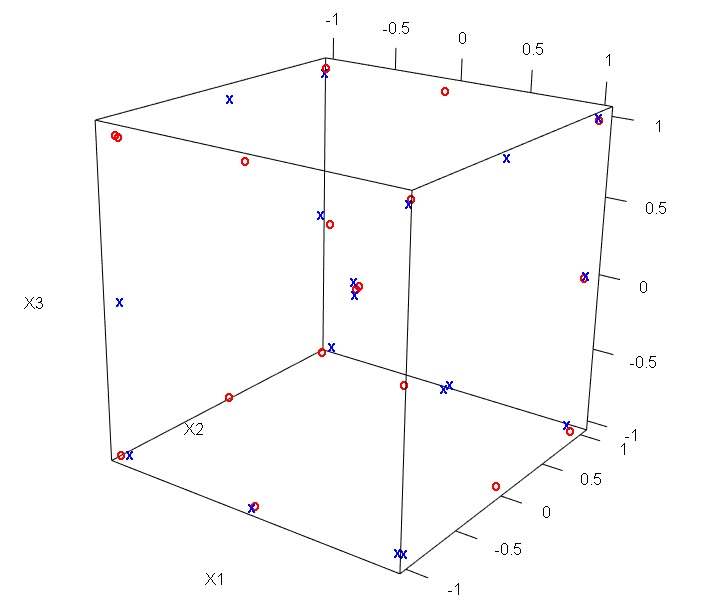
\includegraphics[scale=0.65]{CS_design.jpg}      %width=\textwidth
\caption{MSE(D)-optimal design \#$1$ with two centre points, $\tau^2=1$}
\label{fig::CS_design}
\end{center}
\end{figure} 

Figure \ref{fig::CS_design} provides a graphical representation of the design: the three axes correspond to the experimental factors, each is at three levels (i.e. scaled to $[-1,1]$ dosages): $-1$, $0$ and $1$. Each dot is a design point, and two colours (blue and red) and two symbols (`x' and `o') serve as block indicators. We can see that there are only two centre points in each block, as required, and replicates of other points are generally split between blocks (except for the $(-1,1,1)$ point which is duplicated in the first block only). 

All other designs may be found in the Supplementary material. Time-wise, for the search algorithm's parameters outlined in the beginning of this section, on average an optimal design was found in $13-15$ hours, which was acceptable in this particular case. Sometimes, however, it took up to $20-24$ hours, so some extra time allowance should be accounted for when using these criteria and this search algorithm. 

%%% MSE(D)-optimal designs, WITH centre points: DP, LoF(DPs) and MSE(D) -- LoF as Ds for potential terms
Further we decided to check what designs we would get if there were $5$ levels of each factor rather than $3$, so that all of the third-order terms are estimable (which is also feasible due to a large enough number of runs), i.e. the lack-of-fit component minimising the posterior confidence region for the potential terms would be replaced by the $DP_S$-optimality for them, as in (\ref{eq::crit2}). 

The summary of the corresponding optimal designs is given in Table \ref{tab::MSE(D)_caseCPLoF}: the `new' lack-of-fit component is denoted by DP*s. The notions of `global'  and `local' efficiencies are the same as previously. For each design we calculated its $LoF(DP)$-value, so that we could assess how they would perform in terms of the criterion (\ref{eq::crit1}). The performances of the optimal designs constructed without the restriction of two centre points per block are summarised in Table \ref{tab::MSE(D)_full} in Appendix \ref{app::cs}; all of the designs are also provided in the Supplementary material. In order to illustrate general tendencies in the designs' appearances, designs optimal with respect to the criterion with equal weights, for two values of $\tau^2$ are provided in Table \ref{tab::Full_designs}.

\begin{table}[h]
\centering
\caption{Case-study. Properties of ``Full'' MSE(D)-optimal blocked designs, with two centre points per block}
\label{tab::MSE(D)_caseCPLoF}
\resizebox{\textwidth}{!}}  & \multicolumn{4}{l}{\textbf{`Local' Efficiency,\%}}& \multicolumn{1}{c}{\textbf{Relative}}                          \\
   & \textbf{DP}       & \textbf{DP*s}    & \textbf{MSE(D)}   & \textbf{PE}        & \textbf{LoF}        & \textbf{DP} & \textbf{DP*s}  & \textbf{LoF(DP)}   & \textbf{MSE(D)}  &  \textbf{DP}  &  \textbf{DP*s} & \textbf{LoF(DP)}   & \textbf{MSE(D)} & \textbf{Efficiency,\%} \\
1 & 1/3 & 1/3 & 1/3 & \multicolumn{1}{|r}{14} & \multicolumn{1}{r|}{11} & 80.58 & 69.38 & 87.05 & 91.74 & \multicolumn{1}{|r}{84.46} & 79.90 & 94.36 & \multicolumn{1}{r|}{92.46} & 94.42 \\
2 & 0.4 & 0.2 & 0.4 & \multicolumn{1}{|r}{14} & \multicolumn{1}{r|}{11} & 83.90 & 61.18 & 85.36 & 57.47 & \multicolumn{1}{|r}{87.93} & 70.46 & 92.52 & \multicolumn{1}{r|}{57.92} & 95.83 \\
3 & 0.25 & 0.25 & 0.5 & \multicolumn{1}{|r}{13} & \multicolumn{1}{r|}{12} & 79.93 & 68.24 & 87.06 & 94.05 & \multicolumn{1}{|r}{83.77} & 78.59 & 94.37 & \multicolumn{1}{r|}{94.79} & 96.32 \\
4 & 1 & 0 & 0 & \multicolumn{1}{|r}{20} & \multicolumn{1}{r|}{5} & 95.41 & 0.00 & 62.13 & 95.24 & \multicolumn{1}{|r}{100.00} & 0.00 & 67.34 & \multicolumn{1}{r|}{95.98} & 95.41 \\
5 & 0 & 1 & 0 & \multicolumn{1}{|r}{14} & \multicolumn{1}{r|}{11} & 62.01 & 86.83 & 92.98 & 74.95 & \multicolumn{1}{|r}{64.99} & 100.00 & 100.78 & \multicolumn{1}{r|}{75.53} & 86.83 \\
6 & 0 & 0 & 1 & \multicolumn{1}{|r}{14} & \multicolumn{1}{r|}{11} & 88.31 & 0.00 & 88.35 & 99.23 & \multicolumn{1}{|r}{92.55} & 0.00 & 95.77 & \multicolumn{1}{r|}{100.00} & 99.23 \\
 & & & & & & & & & & & & & & \\
   & \multicolumn{3}{l}{\textbf{Criteria, $\bm{\tau^2=1/q}$}} & \multicolumn{2}{l}{\textbf{DoF}} & \multicolumn{4}{l}{\textbf{`Global' Efficiency,\%}}  & \multicolumn{4}{l}{\textbf{`Local' Efficiency,\%}}& \multicolumn{1}{c}{\textbf{Relative}}                          \\
    & \textbf{DP}       & \textbf{DP*s}    & \textbf{MSE(D)}   & \textbf{PE}   & \textbf{LoF}        & \textbf{DP} & \textbf{DP*s}  & \textbf{LoF(DP)}   & \textbf{MSE(D)}  &  \textbf{DP} & \textbf{DP*s} & \textbf{LoF(DP)}   & \textbf{MSE(D)} & \textbf{Efficiency,\%} \\
1 & 1/3 & 1/3 & 1/3 & \multicolumn{1}{|r}{14} & \multicolumn{1}{r|}{11} & 80.14 & 69.01 & 87.70 & 91.41 & \multicolumn{1}{|r}{83.99} & 81.43 & 90.34 & \multicolumn{1}{r|}{92.07} & 93.97\\
2 & 0.4 & 0.2 & 0.4 & \multicolumn{1}{|r}{14} & \multicolumn{1}{r|}{11} & 83.76 & 61.29 & 88.28 & 94.41 & \multicolumn{1}{|r}{87.79} & 72.31 & 90.95 & \multicolumn{1}{r|}{95.09} & 96.04\\
3 & 0.25 & 0.25 & 0.5 & \multicolumn{1}{|r}{12} & \multicolumn{1}{r|}{13} & 79.66 & 64.43 & 84.44 & 94.84 & \multicolumn{1}{|r}{83.49} & 76.02 & 86.99 & \multicolumn{1}{r|}{95.52} & 95.20\\
4 & 1 & 0 & 0 & \multicolumn{1}{|r}{20} & \multicolumn{1}{r|}{5} & 95.41 & 0.00 & 90.63 & 95.66 & \multicolumn{1}{|r}{100.00} & 0.00 & 93.37 & \multicolumn{1}{r|}{96.35} &  95.41\\
5 & 0 & 1 & 0 & \multicolumn{1}{|r}{14} & \multicolumn{1}{r|}{11} & 59.81 & 84.75 & 86.15 & 72.05 & \multicolumn{1}{|r}{62.68} & 100.00 & 88.75 & \multicolumn{1}{r|}{72.57} & 84.75 \\
6 & 0 & 0 & 1 & \multicolumn{1}{|r}{14} & \multicolumn{1}{r|}{11} & 88.73 & 0.00 & 90.57 & 99.29 & \multicolumn{1}{|r}{92.99} & 0.00 & 93.30 & \multicolumn{1}{r|}{100.00} & 99.29
\end{tabular}
}
\end{table}

\begin{table}[h]
\centering
\caption{Case-study. Designs \#$1$ from Table \ref{tab::MSE(D)_caseCPLoF}, $\tau^2=1$ (left) and $\tau^2=1/q$ (right)}
\begin{center}
\label{tab::Full_designs}
\scalebox{0.73}{
\begin{tabular}{rrrrrrrr|r|rrrrlrrr}
-1 & -1 & 0 &  & -1 & -1 & -1 &  &  &  & -1 & -1 & -1 &  & -1 & -1 & -1 \\
-1 & -1 & 1 &  & -1 & -1 & 0 &  &  &  & -1 & -1 & 0.5 &  & -1 & -1 & 0.5 \\
-1 & 0 & -1 &  & -1 & -1 & 1 &  &  &  & -1 & -0.5 & 1 &  & -1 & -0.5 & 1 \\
-1 & 0.5 & 1 &  & -1 & 0.5 & 1 &  &  &  & -1 & 0 & -0.5 &  & -1 & 1 & -1 \\
-1 & 1 & -1 &  & -1 & 1 & -1 &  &  &  & -1 & 1 & -1 &  & -1 & 1 & 1 \\
-1 & 1 & 0.5 &  & -1 & 1 & 0.5 &  &  &  & -1 & 1 & 1 &  & -0.5 & -1 & -0.5 \\
-0.5 & 1 & 1 &  & -0.5 & -0.5 & 1 &  &  &  & -0.5 & 1 & 0 &  & -0.5 & 0.5 & -1 \\
0 & -1 & -1 &  & -0.5 & 1 & -0.5 &  &  &  & 0 & -1 & 1 &  & 0 & -1 & 1 \\
0 & 0 & 0 &  & 0 & -1 & -1 &  &  &  & 0 & 0 & 0 &  & 0 & 0 & 0 \\
0 & 0 & 0 &  & 0 & 0 & 0 &  &  &  & 0 & 0 & 0 &  & 0 & 0 & 0 \\
0.5 & -1 & 1 &  & 0 & 0 & 0 &  &  &  & 0 & 1 & 1 &  & 0 & 1 & 1 \\
0.5 & 1 & -1 &  & 0.5 & -1 & 1 &  &  &  & 0.5 & -0.5 & -1 &  & 0.5 & 1 & -0.5 \\
1 & -1 & -1 &  & 0.5 & 1 & -1 &  &  &  & 1 & -1 & -1 &  & 1 & -1 & -1 \\
1 & -1 & 0.5 &  & 1 & -1 & -1 &  &  &  & 1 & -1 & 0 &  & \textbf{1} & \textbf{-1} & \textbf{1} \\
1 & -0.5 & 1 &  & 1 & -1 & 0.5 &  &  &  & 1 & 0.5 & 1 &  & \textbf{1} & \textbf{-1} & \textbf{1} \\
1 & 0.5 & -1 &  & 1 & -0.5 & -0.5 &  &  &  & \textbf{1} & \textbf{1} & \textbf{-1} &  & 1 & 0 & -0.5 \\
1 & 1 & -0.5 &  & 1 & 0.5 & -1 &  &  &  & \textbf{1} & \textbf{1} & \textbf{-1} &  & 1 & 0.5 & 1 \\
1 & 1 & 1 &  & 1 & 1 & 1 &  &  &  & 1 & 1 & 0.5 &  & 1 & 1 & 0.5
\end{tabular}
}
\end{center}
\end{table}

In case of $\tau^2=1$ all pure error degrees of freedom (except for the $2$ coming from the replicated centre points) occur from $12$ points duplicated in different blocks; in case of $\tau^2=1/q$ (i.e. $\tau^2=0.1$) two `corner' points are replicated within the same block (they are highlighted in Table \ref{tab::Full_designs}). Quite a few experimental units would receive an `intermediate' $\pm 0.5$ dosage of at least one product, and as this did not comply with the demands of the experimenters, the choice was still made in favour of the three-level design in Table \ref{tab::CS_Design}. 


\section{Future work}


\section{Acknowledgements}

%%% Bibliography
\cleardoublepage
\phantomsection
\addcontentsline{toc}{chapter}{Bibliography} 
%\bibliographystyle{apalike}
\bibliographystyle{rss}
\bibliography{thesis_bib}

\end{document}